%% =====================================================================
%%  PGARA: Profile-Guided Adaptive Register Allocation
%%  IEEE Access manuscript (ieeeaccess.cls).  Compile with:
%%      pdflatex pgara && pdflatex pgara
%%  External files are the GUI screenshots gui_*.png; the manuscript still
%%  compiles (with framed boxes in their place) if they are missing.
%% =====================================================================
\documentclass{ieeeaccess}

\usepackage{cite}
\usepackage{amsmath,amssymb,amsfonts}
\usepackage{stmaryrd}
\usepackage{algorithm}
\usepackage{algorithmic}
\usepackage{graphicx}
\usepackage{textcomp}
\usepackage{xcolor}
\usepackage{booktabs}
\usepackage{multirow}
\usepackage{array}
\usepackage{url}
\usepackage[hidelinks]{hyperref}
\usepackage{tikz}
\usetikzlibrary{arrows.meta,positioning,shapes.geometric,fit,calc,backgrounds}
\usepackage{pgfplots}
\pgfplotsset{compat=1.18}

\definecolor{ink}{HTML}{111827}
\definecolor{card}{HTML}{F3F4F6}
\definecolor{rule}{HTML}{E5E7EB}
\definecolor{mid}{HTML}{6B7280}
\definecolor{indigo}{HTML}{4F46E5}
\definecolor{violet}{HTML}{7C3AED}
\definecolor{emerald}{HTML}{059669}
\definecolor{amber}{HTML}{D97706}
\definecolor{orangeC}{HTML}{EA580C}
\definecolor{rose}{HTML}{DB2777}
\definecolor{sky}{HTML}{0284C7}
\definecolor{redC}{HTML}{DC2626}
\definecolor{slate}{HTML}{64748B}
\definecolor{cPG}{HTML}{6366F1}
\definecolor{cSP}{HTML}{0EA5E9}
\definecolor{cLD}{HTML}{F59E0B}
\definecolor{cLS}{HTML}{64748B}
\definecolor{cFP}{HTML}{10B981}
\definecolor{cCBp}{HTML}{E11D48}

\newtheorem{definition}{Definition}
\newtheorem{proposition}{Proposition}
\newenvironment{proofsketch}{\noindent\textit{Proof sketch.}\ }{\hfill$\square$\par}

\newcommand{\MG}{PGARA}
\newcommand{\Reg}{\mathsf{R}}
\newcommand{\Mem}{\mathsf{M}}
\newcommand{\cld}{c_{\mathrm{ld}}}
\newcommand{\cst}{c_{\mathrm{st}}}
\newcommand{\csv}{\sigma}
\newcommand{\cmv}{c_{\mathrm{mv}}}
\newcommand{\First}{\mathrm{FIRST}}
\newcommand{\Follow}{\mathrm{FOLLOW}}
\newcommand{\nt}[1]{\textit{#1}}
\newcommand{\tm}[1]{\texttt{#1}}

\tikzset{
  stage/.style={draw=sky, rounded corners=2pt, fill=sky!8, align=center, line width=0.6pt,
                font=\scriptsize, minimum height=7.5mm, inner sep=2pt},
  midst/.style={stage, draw=emerald, fill=emerald!9},
  hot/.style={stage, draw=indigo, top color=indigo, bottom color=violet, text=white},
  back/.style={stage, draw=amber, fill=amber!10},
  flow/.style={-{Stealth[length=1.6mm]}, draw=ink!80, line width=0.55pt},
  soft/.style={-{Stealth[length=1.4mm]}, draw=violet!70, dashed, line width=0.5pt},
  blk/.style={draw=slate, rounded corners=1.5pt, fill=white, align=left,
              font=\scriptsize\ttfamily, inner sep=2.5pt},
}

\begin{document}
\newlength{\xfigwd}
\setlength{\xfigwd}{\columnwidth}

\history{Date of publication xxxx 00, 0000, date of current version xxxx 00, 0000.}
\doi{10.1109/ACCESS.2026.DOI}

\title{PGARA: Profile-Guided Adaptive Register Allocation via Markov
Decision Processes and Game-Theoretic Auctions}

\author{\uppercase{Shreyans Chowdry}\authorrefmark{1},
\uppercase{Samrender Singh Saini}\authorrefmark{1},
\uppercase{Karthikeya Jami}\authorrefmark{1},
\uppercase{Abhishek Kumar}\authorrefmark{1}, and
\uppercase{Nishanth Kumar}\authorrefmark{1}}

\address[1]{School of Computer Science and Engineering, Vellore Institute
of Technology, Vellore, Tamil Nadu 632014, India (e-mail:
shreyans.chowdry2024@vitstudent.ac.in;
samrender.singh2024@vitstudent.ac.in;
jami.karthikeya2024@vitstudent.ac.in;
abhishek.kumar2024b@vitstudent.ac.in;
akula.nishanthkumar2024@vitstudent.ac.in)}

\tfootnote{This work received no external funding.}

\markboth
{Chowdry \headeretal: PGARA: Profile-Guided Adaptive Register Allocation}
{Chowdry \headeretal: PGARA: Profile-Guided Adaptive Register Allocation}

\corresp{Corresponding author: Shreyans Chowdry (e-mail: shreyans.chowdry2024@vitstudent.ac.in).}

\begin{abstract}
The register allocator decides which values a compiler keeps in a
processor's few registers, and the right decision depends on how often
each path through the program is actually taken. Production allocators
rank spill candidates by access counts weighted by loop depth or, with a
profile, by block frequency; learned allocators train opaque policies on
large corpora. We present PGARA (Profile-Guided Adaptive Register
Allocation), which models the residency of every SSA value as a
two-state Markov decision process over the control-flow graph with
profiled transition probabilities. Policy evaluation yields each value's
expected cycles saved under the policy the code generator realises;
values on a loop-carried $\varphi$-web bid as one coalition; registers
are sold in a sealed-bid auction along a maximum-cardinality-search
order of the chordal SSA interference graph; and best-response dynamics
reach a pure Nash equilibrium. PGARA is embedded in a complete compiler
for a C subset, from a DFA lexer and LL(1) parser to SSA optimisation,
code generation and a cycle-counting simulator, with a web interface
that visualises every phase. On 17 programs, seven of them translated
from MiBench and BEEBS, and register budgets from 3 to 32, all 1{,}428
configurations reproduce the reference output. At four registers PGARA
lowers geometric-mean cycles by 21.8\% relative to linear scan, 3.7\%
relative to Chaitin--Briggs colouring with profile-weighted spill costs,
3.3\% relative to profile-weighted priority allocation and 2.6\%
relative to static branch priors, and halves spill traffic relative to
linear scan. The benefit is stable across test inputs, confined to
budgets of eight registers or fewer, and requires a representative
profile.
\end{abstract}

\begin{keywords}
Compiler design, game theory, Markov decision process,
profile-guided optimisation, register allocation, static single
assignment.
\end{keywords}

\titlepgskip=-15pt

\maketitle

\section{Introduction}
\label{sec:intro}

\PARstart{C}{ompilers} are the bridge between the abstractions programmers write and
the narrow interface that hardware executes. Their structure has been
stable for decades (a front end that recognises and checks the
language, a middle end that transforms a machine-independent
intermediate representation, and a back end that maps it to
instructions and registers), but the techniques inside each phase keep
evolving, from reusable multi-level infrastructures such as
MLIR~\cite{lattner2021mlir} to optimisation heuristics learned from
data~\cite{wang2018ml,ashouri2018survey,leather2020ml}. Static single
assignment (SSA) form~\cite{cytron1991ssa,rastello2022ssa} is now the
common currency of this middle end, and the textbooks used to teach the
subject treat it as such~\cite{cooper2022eac,aho2006dragon}.

Among back-end problems, register allocation has an outsized effect on
performance: a value that is not kept in a register costs a store when
it is produced and a load each time it is consumed, and on a loop that
runs millions of times these accesses dominate execution time. The
problem is hard for two reasons. First, the decision is combinatorial,
since values that are live at the same time compete for the same $k$
registers. Second, the payoff of each decision is uncertain at compile
time, because it depends on which branches the program actually takes.
A value used only on an error path that runs once in a thousand
iterations is worth far less than one used on the hot path, yet a
static analysis sees the two paths as symmetric. Our motivation is to
treat this second difficulty as a first-class modelling concern rather
than a tuning detail.

Existing allocators fall broadly into three families. Graph-colouring
allocators, descending from Chaitin~\cite{chaitin1982} and the
priority-based variant of Chow and Hennessy~\cite{chow1990}, build an
interference graph and colour it with $k$ colours, choosing spill
candidates by a cost that weights each access by an execution-frequency
estimate: classically $10^{d}$ for loop depth $d$, and in production
compilers such as LLVM's greedy allocator the estimated block frequency,
which reflects measured counts when profile-guided optimisation is
enabled~\cite{olesen2011greedy,llvmbfi}. Linear-scan allocators~\cite{poletto1999} trade quality for speed
by sweeping live intervals in program order. On SSA form the
interference graph is chordal~\cite{hack2006ssa,hack2006ipl}, which makes
colouring itself polynomial and moves the difficulty entirely into the
spilling decision; combinatorial approaches solve allocation and
scheduling jointly to proven optimality~\cite{lozano2019toplas,lozano2019survey}.

A newer family learns allocation and related decisions from data.
MLGO~\cite{trofin2021mlgo} trains policies inside LLVM's production
allocator, RL4ReAl~\cite{venkatakeerthy2023rl4real} learns end-to-end
register allocation with reinforcement learning over embeddings such as
IR2Vec~\cite{venkatakeerthy2020ir2vec}, and environments such as
CompilerGym~\cite{cummins2022compilergym} and representations such as
ProGraML~\cite{cummins2021programl} make these experiments
reproducible. In parallel, profile-guided post-link optimisers such as
BOLT~\cite{panchenko2019bolt} and Propeller~\cite{shen2023propeller}
have shown that measured execution profiles yield large gains in code
layout, and recent work predicts profiles when none are
available~\cite{rotem2021pgo}.

These families leave a gap. Spill weights built from static estimates
encode a fixed belief about branch behaviour (loops iterate about ten
times; both arms of a conditional are equally likely), so they mis-rank
values precisely on programs with data-dependent control flow, as early
studies of static estimators already observed~\cite{wagner1994,wu1994,wall1991}.
When a profile is available, production compilers already scale spill
costs by measured block frequencies~\cite{olesen2011greedy,llvmbfi},
and frequency-weighted spill costs go back to hierarchical and
progressive allocators~\cite{callahan1991,koes2006}. Such
profile-weighted costs remove the fixed belief, but they still rank a
value by a frequency-weighted count of its accesses: they do not model
the value's residency over its live range (where a spill or reload
would occur, what calls cost, which loads the peephole pass forwards),
they do not make loop-carried $\varphi$-webs bid as one, and the
heuristic that applies them (simplify, spill, evict) leaves the
objective implicit. Whether modelling these effects is worth more than
simply weighting accesses by measured frequency is an empirical
question that this paper tests directly. Learned policies
avoid fixed beliefs, but they require large training corpora and
expensive training loops~\cite{sutton2018rl}, and the decision they make
for a particular value cannot be traced back to a quantity a compiler
engineer can inspect.

Classical colouring formulations also obscure the objective. A
colouring is either feasible or not, and the quality of the result
emerges indirectly from the order in which nodes are simplified and
spilled. Neither family states, for each value, the expected number of
cycles that keeping it in a register will save.

We propose \MG\ (Profile-Guided Adaptive Register Allocation), which
makes that expected saving the central quantity. It is profile-guided
because every probability it uses is measured on a training run, and
adaptive because the same program receives a different allocation when
its measured behaviour changes, without any hand-tuned weights.
Each SSA value's residency is a two-state Markov decision process (MDP)
over its live range in the control-flow graph~\cite{puterman1994,bertsekas2019};
transition probabilities are measured edge frequencies, and exact policy
iteration~\cite{howard1960} gives the value's expected gain per
invocation. Allocation is then a resource-contention game: values that
form a loop-carried $\varphi$-web bid together as a coalition, in the
spirit of cooperative game theory~\cite{shapley1953}, registers are sold
in a sealed-bid auction~\cite{vickrey1961} processed along a
maximum-cardinality-search (MCS) order~\cite{tarjan1984} of the chordal
interference graph, and best-response dynamics settle the result into a
pure Nash equilibrium~\cite{rosenthal1973,nisan2007agt}. The approach
is apt because each ingredient matches a structural fact of the problem:
SSA makes the contention structure chordal, profiles make the
uncertainty measurable, and the gain is an explicit, inspectable number.

The advantages are practical as well as conceptual. Policy iteration on
a two-state MDP per value converges in about 1.3 improvement rounds on
average, so allocation takes milliseconds; every decision can be
explained by a bid and an auction round; and the same engine runs
unchanged on static priors, which isolates the value of profiling.
To evaluate it honestly we built a complete compiler around it, from a
formally specified grammar to a cycle-counting simulator, and a web
interface that renders every intermediate artefact.

\textit{Contributions.} The main contribution is the \emph{gain
formulation}: modelling the register residency of each SSA value as a
two-state MDP over its live range, with measured branch probabilities,
and using its exact solution, the expected cycles saved per invocation,
as the quantity that every allocation decision is based on. The
remaining parts adapt known ideas, and we credit them as such: the
chordality of SSA interference graphs and maximum cardinality
search~\cite{hack2006ssa,tarjan1984}, coalescing of $\varphi$-related
values (here as coalitions that bid together), a capacity-$k$
sealed-bid auction that is solved by sorting, best-response
dynamics~\cite{nisan2007agt}, and edge profiling with static
fallbacks~\cite{wu1994}. A secondary contribution is the evaluation
vehicle itself: a complete, tested compiler and web interface in which
every allocator shares the same front end, interference graph and code
generator, so that differences between allocators are attributable to
the allocation decision alone.

\textit{Research questions.} The evaluation answers four questions:
\begin{itemize}
\item[RQ1] Does profiling help? Is \MG\ with measured probabilities
better than the same engine driven by static priors?
\item[RQ2] Does the MDP and auction formulation help beyond profiling?
Is \MG\ better than simply weighting accesses by profiled block
frequency, and better than graph colouring with profile-weighted
spill costs?
\item[RQ3] How robust are the results to the register budget (up to
$k=32$), to independently written programs, to several test inputs, to
the quality of the training profile and to the model constants?
\item[RQ4] What does it cost at compile time, including the profiling
run, and how does that cost grow with function size?
\end{itemize}
Section~\ref{sec:rq} answers each question explicitly.

The remainder of the paper is organised as follows.
Section~\ref{sec:related} reviews fifteen recent works, and the
classical work on frequency-based spill costs, and the gaps they leave. Section~\ref{sec:proposed} formalises the language, the front
end, the intermediate representations and the optimiser, then develops
the MDP, the gain, the coalitions and the auction, with the algorithms
and their properties. Section~\ref{sec:impl} describes the toolchain,
the parameters and the results on five metrics against six baselines,
followed by the ablations, robustness studies and answers to the
research questions.
Section~\ref{sec:conclusion} concludes, and the team's contributions are
listed after it.

%% =====================================================================
\section{Related Works}
\label{sec:related}

We review fifteen works from 2018--2025, grouped by theme, followed by
the older line of work on frequency-based spill costs that is closest
to \MG. For each we summarise the proposed solution, its methodology
and tools, the reported effectiveness and the research gap relative to
\MG.

\subsection{Combinatorial and survey work on allocation}

\textit{Castañeda Lozano et~al.}~\cite{lozano2019toplas} propose Unison,
which formulates global register allocation (including spilling,
coalescing and live-range splitting) together with instruction
scheduling as a single constraint model. Programs are first transformed
into linear SSA, the model is solved with a constraint programming
solver using problem-specific decomposition, and it is integrated with
LLVM for Hexagon, ARM and MIPS. Unison produces provably optimal or
near-optimal code for functions of up to about a thousand instructions
and improves on LLVM's heuristics for a measurable fraction of them.
\textit{Gap:} the objective is a static cost estimate, and solve times
grow quickly with function size.

\textit{Castañeda Lozano and Schulte}~\cite{lozano2019survey} survey
combinatorial approaches to register allocation and instruction
scheduling. They classify integer programming, constraint programming,
PBQP and related models by the subproblems covered, by scalability and
by the quality of the code produced, and compare reported evaluations
across targets. The survey shows that combinatorial methods reach
optimality on medium-sized functions but are seldom used in production.
\textit{Gap:} almost all surveyed models assume static frequency
estimates rather than measured, stochastic behaviour.

\subsection{Learning-based allocation and program representation}

\textit{VenkataKeerthy et~al.}~\cite{venkatakeerthy2023rl4real} present
RL4ReAl, a reinforcement-learning register allocator. The interference
graph is embedded with IR2Vec features and a hierarchy of agents learns
to pick nodes to colour, spill or split, trained with policy-gradient
methods inside an LLVM-based gRPC environment for x86 and AArch64. The
learned allocator matches or improves on LLVM's greedy allocator on
several benchmark suites. \textit{Gap:} training is costly and
individual decisions are not interpretable as expected savings.

\textit{Trofin et~al.}~\cite{trofin2021mlgo} introduce MLGO, a framework
for integrating trained policies in LLVM. Policies for inlining-for-size
and, later, register-allocation eviction are trained offline with
reinforcement learning and evolution strategies on corpora of production
code and shipped as compiled TensorFlow models. Inlining-for-size
achieved several percent size reduction on large binaries.
\textit{Gap:} policies generalise from a corpus, not from the profile of
the program being compiled.

\textit{Cummins et~al.}~\cite{cummins2022compilergym} present
CompilerGym, a set of environments that expose compiler optimisation
problems through the OpenAI Gym interface. It wraps LLVM phase ordering,
GCC flag tuning and loop-nest generation behind a client-server
architecture, with datasets of millions of programs and multiple
observation spaces. It made reinforcement-learning experiments on
compilers reproducible and fast. \textit{Gap:} it targets pass-level
decisions, not per-value register decisions.

\textit{Cummins et~al.}~\cite{cummins2021programl} propose ProGraML, a
graph representation of programs that combines control, data and call
flow, processed by gated graph neural networks. The representation is
built from LLVM and XLA IR and evaluated on data-flow analyses and
heuristics such as device mapping and thread coarsening. It
outperformed sequence-based representations on those tasks.
\textit{Gap:} it learns to approximate analyses that \MG\ computes
exactly.

\textit{VenkataKeerthy et~al.}~\cite{venkatakeerthy2020ir2vec} introduce
IR2Vec, distributed embeddings of LLVM IR derived from a learned
seed-embedding vocabulary and flow analysis. Embeddings are computed at
instruction, function and program level without heavy training, and used
for heterogeneous device mapping and thread-coarsening prediction with
competitive accuracy. \textit{Gap:} embeddings capture syntax and flow,
not execution frequencies.

\textit{Jain et~al.}~\cite{jain2022posetrl} propose POSET-RL, which
orders optimisation passes with reinforcement learning. A partially
ordered set of pass sub-sequences derived from LLVM's O-levels defines
the action space, and a deep Q-network trained on IR2Vec states optimises
size and execution time. It reduced code size and runtime relative to
the standard pipeline on SPEC and MiBench. \textit{Gap:} it operates
above the allocator and treats it as a black box.

\textit{Haj-Ali et~al.}~\cite{hajali2020neurovectorizer} present
NeuroVectorizer, which learns vectorisation and interleaving factors
with deep reinforcement learning. Loops are embedded with code2vec and a
policy chooses pragmas that Clang/LLVM applies, with rewards measured by
execution time. It outperformed the baseline cost model on a range of
loop kernels. \textit{Gap:} measured rewards drive training, but the
decision is not grounded in a model of the program's behaviour.

\subsection{Surveys of machine learning in compilers}

\textit{Wang and O'Boyle}~\cite{wang2018ml} survey machine learning in
compiler optimisation. They organise the field by feature engineering,
learning models and deployment, covering search-based tuning,
predictive modelling and deep learning across many published systems,
and show consistent gains over hand-written heuristics.
\textit{Gap:} register allocation is barely represented, and the role of
measured profiles inside heuristics is left open.

\textit{Ashouri et~al.}~\cite{ashouri2018survey} survey compiler
autotuning with machine learning, with an emphasis on optimisation
selection and phase ordering. They classify works by learning model,
features and prediction type and summarise the tools used, from
Milepost-GCC to LLVM-based frameworks, reporting the speed-ups achieved.
\textit{Gap:} the focus is on choosing passes, not on resource
assignment inside a pass.

\subsection{Profile-guided optimisation}

\textit{Panchenko et~al.}~\cite{panchenko2019bolt} present BOLT, a
post-link optimiser that uses sampled hardware profiles. It rewrites
binaries using LLVM's MC infrastructure and reorders basic blocks and
functions according to Linux \texttt{perf} profiles collected in
production. It gave substantial speed-ups on large data-centre
applications already built with feedback-directed optimisation.
\textit{Gap:} it uses profiles for layout only; register decisions are
fixed before it runs.

\textit{Shen et~al.}~\cite{shen2023propeller} present Propeller, a
profile-guided relinking optimiser for warehouse-scale applications. It
integrates profile-driven basic-block layout into the build through
distributed, incremental relinking with the LLVM toolchain, avoiding
BOLT's monolithic binary rewrite. It achieved comparable speed-ups with
much lower memory and build-time cost. \textit{Gap:} as with BOLT, the
relinker does not revisit register decisions; inside the compiler the
profile reaches allocation only as block-frequency weights on spill
costs (Section~\ref{sec:freqrw}).

\textit{Rotem and Cummins}~\cite{rotem2021pgo} predict branch
probabilities statically so that profile-guided optimisation can run
without profiles. A gradient-boosted model is trained on features of
branches in a large corpus of profiled code and its predictions are fed
into LLVM's PGO pipeline. A substantial share of the benefit of real
profiles was recovered. \textit{Gap:} predicted probabilities feed
existing static heuristics rather than an allocation model that uses
them directly.

\subsection{Infrastructure and large language models}

\textit{Lattner et~al.}~\cite{lattner2021mlir} introduce MLIR, a
multi-level compiler infrastructure with extensible dialects, regions
and SSA-based IR that is shared across domains. It is implemented in
C++ within the LLVM project and used to build compilers for machine
learning, hardware design and more. It reduced the cost of building
domain-specific compilers. \textit{Gap:} MLIR lowers to LLVM's
allocators and does not change how registers are assigned.

\textit{Cummins et~al.}~\cite{cummins2025llmcompiler} present LLM
Compiler, a family of foundation models for compiler optimisation. Code
models are further trained on a large corpus of LLVM IR and assembly to
emulate the compiler, then fine-tuned to choose optimisation pass
lists for code size and to disassemble machine code back into IR. The
models recover a substantial share of the code-size savings of an
autotuning search without any additional compilations, and they are
released for further research. \textit{Gap:} their outputs are not
guaranteed correct and give no account of the decisions made.

\subsection{Frequency-based spill costs and profile-guided allocation}
\label{sec:freqrw}

This line of work is the closest to \MG's central idea, and we review
it separately because it predates the 2018--2025 window.
\textit{Wall}~\cite{wall1991} compared real and estimated profiles as
inputs to optimisations including link-time register allocation, and
found that estimated profiles recover only part of the benefit of
measured ones. \textit{Callahan and Koblenz}~\cite{callahan1991}
colour a hierarchy of tiles that follows the program structure and use
execution-frequency estimates to place spill code in infrequently
executed tiles. \textit{Briggs et~al.}~\cite{briggs1994} and
\textit{George and Appel}~\cite{george1996} established optimistic
colouring and conservative and iterated coalescing, with spill costs
weighted by estimated frequency, which is the form of graph-colouring
allocator we use as a baseline. \textit{Lueh et~al.}~\cite{lueh2000}
allocate regions in order of their execution frequency and fuse them,
and \textit{Koes and Goldstein}~\cite{koes2006} formulate global
allocation as a multi-commodity network-flow problem whose costs are
weighted by expected execution frequency and refine it progressively.
In LLVM, the greedy allocator computes the spill weight of a live range
from the block frequencies of its uses and definitions~\cite{olesen2011greedy},
and those frequencies are derived from profile data when it is
supplied~\cite{llvmbfi}. \textit{Gap:} in all of these, the profile
scales an access count; none states, per value, the expected cycles
that residency saves under a model of spills, reloads, calls and
forwarding, and none makes loop-carried values bid as a coalition.
Section~\ref{sec:ablation} tests whether this difference matters by
comparing \MG\ with a profile-weighted priority allocator and with
Chaitin--Briggs colouring using profile-weighted spill costs.

\subsection{Summary of gaps}

Across these works, measured execution frequencies drive code layout,
and inside the allocator they enter only as weights on spill costs;
learned allocators require heavy training and are opaque; and
combinatorial allocators optimise static cost models. \MG\ addresses
the intersection: an allocator whose objective is the expected saving
under measured probabilities, solved exactly and cheaply, with every
decision explainable as a bid.

%% =====================================================================
\section{Proposed Work}
\label{sec:proposed}

\subsection{Problem formulation}

Let a function in SSA form have values $V$, a control-flow graph (CFG)
$\mathcal{C}=(B,E,b_0)$ and a register file of $k$ registers. An
allocation is a map $\rho: V \to \{0,\dots,k{-}1\}\cup\{\bot\}$ in which
$\rho(v)=\bot$ means that $v$ lives in its stack slot; it is feasible
when no two interfering values share a register. Executing the program
on an input induces a random walk over $\mathcal{C}$, and the cost of
the allocation is the expected number of cycles spent on loads, stores
and copies caused by values without a register. We seek
\begin{equation}
\rho^\star \;=\; \arg\max_{\rho\ \text{feasible}}\;
\sum_{v:\,\rho(v)\neq\bot} G(v),
\label{eq:objective}
\end{equation}
where $G(v)$ is the expected cycles saved by giving $v$ a register,
computed under transition probabilities measured by profiling.

Two features make (\ref{eq:objective}) tractable without colouring.
On strict SSA form the interference graph is chordal~\cite{hack2006ssa},
so the values competing at any program point form a clique that an MCS
order exposes one at a time. And the gain of a single value can be
computed exactly by stochastic dynamic programming over its live range,
because the residency of one value is a small MDP whose only uncertainty
is the branch behaviour of the CFG. Both observations are developed
below, after the front end and middle end that produce the SSA program.

\subsection{System architecture}

Fig.~\ref{fig:arch} shows the architecture. The front end turns MiniC
source text into a type-checked abstract syntax tree (AST) and symbol
table; the middle end lowers it to three-address code (TAC), builds the
CFG, constructs SSA and optimises it; a reference interpreter executes
the optimised SSA on a training input and records edge counts; the
\MG\ engine converts those counts into gains, coalitions and an
auctioned allocation; and the back end leaves SSA, emits PG-RISC code
and runs it on a cycle-counting simulator on a separate test input.

Every stage reports its result into a single JSON document, which the
web interface renders as token streams, AST, symbol tables, TAC, SSA,
CFG, interference graph, auction rounds and target code (dashed arrows
in Fig.~\ref{fig:arch}). Three baseline allocators share the same
pipeline and code generator, so differences in the measured cycles
are attributable to allocation decisions alone.

\begin{figure*}[!t]
\centering
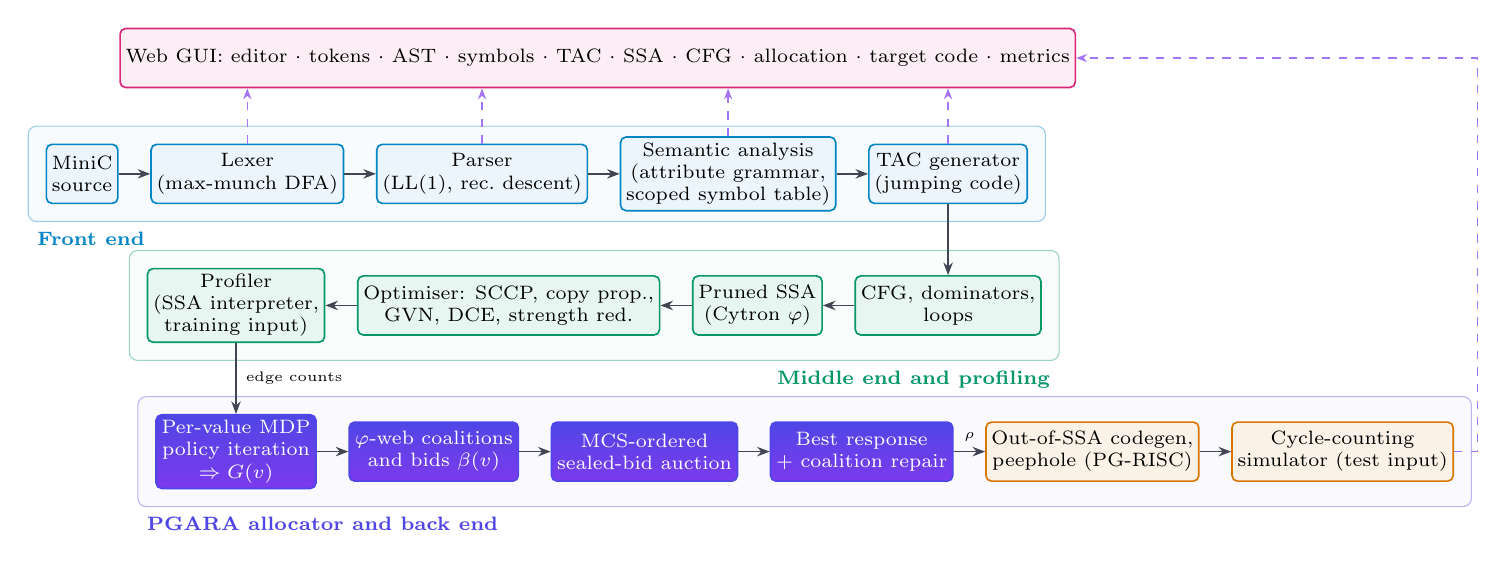
\begin{tikzpicture}[node distance=4.5mm and 4mm]
  % Front end
  \node[stage] (src) {MiniC\\source};
  \node[stage, right=of src] (lex) {Lexer\\(max-munch DFA)};
  \node[stage, right=of lex] (par) {Parser\\(LL(1), rec.\ descent)};
  \node[stage, right=of par] (sem) {Semantic analysis\\(attribute grammar,\\scoped symbol table)};
  \node[stage, right=of sem] (tac) {TAC generator\\(jumping code)};
  % Middle end
  \node[midst, below=9mm of tac] (cfg) {CFG, dominators,\\loops};
  \node[midst, left=of cfg] (ssa) {Pruned SSA\\(Cytron $\varphi$)};
  \node[midst, left=of ssa] (opt) {Optimiser: SCCP, copy prop.,\\GVN, DCE, strength red.};
  \node[midst, left=of opt] (prof) {Profiler\\(SSA interpreter,\\training input)};
  % PGARA allocator
  \node[hot, below=9mm of prof] (mdp) {Per-value MDP\\policy iteration\\$\Rightarrow G(v)$};
  \node[hot, right=of mdp] (coal) {$\varphi$-web coalitions\\and bids $\beta(v)$};
  \node[hot, right=of coal] (auc) {MCS-ordered\\sealed-bid auction};
  \node[hot, right=of auc] (br) {Best response\\+ coalition repair};
  \node[back, right=of br] (cg) {Out-of-SSA codegen,\\peephole (PG-RISC)};
  \node[back, right=of cg] (sim) {Cycle-counting\\simulator (test input)};
  % GUI
  \node[stage, draw=rose, fill=rose!8, above=7mm of $(lex.north)!0.5!(tac.north)$, minimum width=95mm] (gui)
       {Web GUI: editor $\cdot$ tokens $\cdot$ AST $\cdot$ symbols $\cdot$ TAC $\cdot$ SSA $\cdot$ CFG $\cdot$ allocation $\cdot$ target code $\cdot$ metrics};
  \draw[flow] (src) -- (lex);
  \draw[flow] (lex) -- (par);
  \draw[flow] (par) -- (sem);
  \draw[flow] (sem) -- (tac);
  \draw[flow] (tac) -- (cfg);
  \draw[flow] (cfg) -- (ssa);
  \draw[flow] (ssa) -- (opt);
  \draw[flow] (opt) -- (prof);
  \draw[flow] (prof) -- node[right,font=\tiny]{edge counts} (mdp);
  \draw[flow] (mdp) -- (coal);
  \draw[flow] (coal) -- (auc);
  \draw[flow] (auc) -- (br);
  \draw[flow] (br) -- node[above,font=\tiny]{$\rho$} (cg);
  \draw[flow] (cg) -- (sim);
  \draw[soft] (sem.north) -- (sem.north |- gui.south);
  \draw[soft] (par.north) -- (par.north |- gui.south);
  \draw[soft] (lex.north) -- (lex.north |- gui.south);
  \draw[soft] (tac.north) -- (tac.north |- gui.south);
  \draw[soft] (sim.east) -- ++(3mm,0) |- (gui.east);
  \begin{scope}[on background layer]
    \node[draw=sky!40, fill=sky!3, rounded corners=3pt, inner sep=2.2mm,
          fit=(src)(tac), label={[font=\scriptsize\bfseries,text=sky,anchor=north west]south west:Front end}] {};
    \node[draw=emerald!40, fill=emerald!3, rounded corners=3pt, inner sep=2.2mm,
          fit=(prof)(cfg), label={[font=\scriptsize\bfseries,text=emerald,anchor=north east]south east:Middle end and profiling}] {};
    \node[draw=indigo!40, fill=indigo!3, rounded corners=3pt, inner sep=2.2mm,
          fit=(mdp)(sim), label={[font=\scriptsize\bfseries,text=indigo,anchor=north west]south west:\MG\ allocator and back end}] {};
  \end{scope}
\end{tikzpicture}
\caption{Architecture of the \MG\ compiler: front end (blue), middle
end and profiling (green), the \MG\ allocation engine (indigo) and back
end (amber). Dashed violet arrows show phase reports consumed by the web
interface (pink).}
\label{fig:arch}
\end{figure*}

\subsection{Front end: language, grammar and parsing}

\paragraph*{Lexical analysis}
MiniC has \tm{int} scalars and one-dimensional arrays, array parameters
passed by reference, functions, \tm{if}/\tm{else}, \tm{while},
\tm{for}, \tm{break}, \tm{continue}, \tm{print} and \tm{input()}, the
arithmetic, relational and short-circuit logical operators, and the
compound forms \tm{+=}, \tm{-=}, \tm{*=}, \tm{++}, \tm{--}. The lexer is
a deterministic finite automaton applied under the maximal-munch rule:
from position $i$ it returns the longest prefix $w$ of the remaining
input with $\delta^\ast(q_0,w)\in F$, so \tm{<=} is one token and
\tm{a+++b} is \tm{a ++ + b}. Keywords are recognised as identifiers and
reclassified by table lookup. An invalid character is reported with its
line and column and skipped (panic mode), so later errors are still
found in the same run.

\paragraph*{Context-free grammar}
The syntax is the context-free grammar
\begin{equation}
G=(N,\Sigma,P,S),\quad |N|=41,\ |P|=94,\ S=\nt{Program},
\label{eq:grammar}
\end{equation}
written directly in LL(1) form. Left recursion is removed by the
standard tail transformation and precedence is encoded by one
nonterminal per level, for example
\begin{align*}
\nt{Add} &\to \nt{Mul}\ \nt{AddRest}\\
\nt{AddRest} &\to \tm{+}\ \nt{Mul}\ \nt{AddRest} \mid
                \tm{-}\ \nt{Mul}\ \nt{AddRest} \mid \varepsilon\\
\nt{Stmt} &\to \tm{if (}\ \nt{Expr}\ \tm{)}\ \nt{Stmt}\ \nt{ElsePart}\\
          &\phantom{{}\to{}} \mid \tm{while (}\ \nt{Expr}\ \tm{)}\ \nt{Stmt} \mid \cdots\\
\nt{ElsePart} &\to \tm{else}\ \nt{Stmt} \mid \varepsilon .
\end{align*}
The precedence chain, from loosest to tightest binding, is
\nt{Or}, \nt{And}, \nt{Eq}, \nt{Rel}, \nt{Add}, \nt{Mul}, \nt{Unary},
\nt{Primary}, giving the usual C precedence and left associativity.

\paragraph*{FIRST, FOLLOW and the LL(1) property}
For $\alpha\in(N\cup\Sigma)^\ast$ and $A\in N$,
\begin{equation}
\begin{aligned}
\First(\alpha) &= \{a\in\Sigma \mid \alpha \Rightarrow^\ast a\beta\}
                  \cup \{\varepsilon \mid \alpha\Rightarrow^\ast\varepsilon\},\\
\Follow(A) &= \{a\in\Sigma\cup\{\$\} \mid S\$ \Rightarrow^\ast \beta A a \gamma\}.
\end{aligned}
\label{eq:firstfollow}
\end{equation}
Both are computed as least fixpoints of the usual inclusion constraints.
$G$ is LL(1) iff for every pair of alternatives $A\to\alpha\mid\beta$
\begin{equation}
\First\big(\alpha\,\Follow(A)\big)\cap\First\big(\beta\,\Follow(A)\big)=\emptyset .
\label{eq:ll1}
\end{equation}
The toolchain computes (\ref{eq:firstfollow}), builds the predictive
table and checks (\ref{eq:ll1}) mechanically. The single conflict is
the cell (\nt{ElsePart}, \tm{else}): \tm{else} is in $\First(\tm{else}\
\nt{Stmt})$ and, because \nt{ElsePart} can end a \nt{Stmt}, also in
$\Follow(\nt{ElsePart})$. This is the dangling-else ambiguity, resolved
by preferring $\nt{ElsePart}\to\tm{else}\ \nt{Stmt}$ so that an
\tm{else} binds to the nearest unmatched \tm{if}. Every other cell holds
at most one production, so $G$ is LL(1) modulo this resolution.

\paragraph*{Relation to LR parsing}
Every LL(1) grammar is also LR(1)~\cite{knuth1965lr,lewis1968}, so an
LR(1) or LALR parser generator would accept $G$ unchanged apart from the
same dangling-else conflict, which appears there as a shift/reduce
conflict on \tm{else} and is conventionally resolved in favour of
shift, binding \tm{else} the same way. We chose top-down predictive
parsing because a recursive-descent parser is a direct transcription of
the grammar (one procedure per nonterminal), errors can be reported in
terms of the construct being parsed, and the GUI can show the
predictive table, which students can check against
(\ref{eq:firstfollow})--(\ref{eq:ll1}). The parser recovers from syntax
errors in panic mode, discarding tokens until one in the FOLLOW set of
the current construct (for statements, \tm{;} or \tm{\}}) is found.

\subsection{Semantic analysis as an attribute grammar}

Semantic analysis is specified as an L-attributed grammar~\cite{knuth1968attr}
and implemented as a traversal of the AST. Each node carries an
inherited environment $\Gamma$ (a stack of scopes, each a hash map from
names to symbols) and a synthesised type
$\tau\in\{\tm{int},\tm{int[]},\tm{void}\}$. Typical rules are
\begin{equation}
\begin{aligned}
&\nt{Add}\to\nt{Mul}\ \nt{AddRest}:\\
&\quad \nt{AddRest}.\mathit{in}=\nt{Mul}.\mathit{node},\ \
       \nt{Add}.\mathit{node}=\nt{AddRest}.\mathit{out}\\
&\nt{AddRest}\to\tm{+}\ \nt{Mul}\ \nt{AddRest}_1:\\
&\quad \nt{AddRest}_1.\mathit{in}=\mathrm{Bin}(\tm{+},\nt{AddRest}.\mathit{in},\nt{Mul}.\mathit{node}),\\
&\quad \nt{AddRest}.\mathit{out}=\nt{AddRest}_1.\mathit{out}\\
&\nt{AddRest}\to\varepsilon:\quad \nt{AddRest}.\mathit{out}=\nt{AddRest}.\mathit{in}\\
&E\to E_1\ \mathit{op}\ E_2:\quad E.\tau=\tm{int}\ \text{iff}\ E_1.\tau=E_2.\tau=\tm{int}\\
&\nt{Primary}\to\tm{ID}:\quad \nt{Primary}.\tau=\Gamma(\tm{ID}).\tau\ \text{(error if unbound)}
\end{aligned}
\label{eq:attr}
\end{equation}
The inherited attribute $\mathit{in}$ restores left associativity that
the LL(1) transformation removed from the syntax. Fig.~\ref{fig:ast}
shows the flow of attributes on a small statement. Declarations
extend $\Gamma$ in the innermost scope and reject redeclaration in the
same scope; uses resolve outward through enclosing scopes. Functions
are collected in a first pass, so calls may precede definitions. The
analyser checks arity and argument kinds, array indexing and
assignment, use of \tm{void} results, \tm{break}/\tm{continue} outside
loops and missing returns. Every symbol receives a unique IR name: its
own name, or $x\#n$ when that name is already used in the function, so
shadowed variables never collide in later phases.

\begin{figure}[t]
\centering
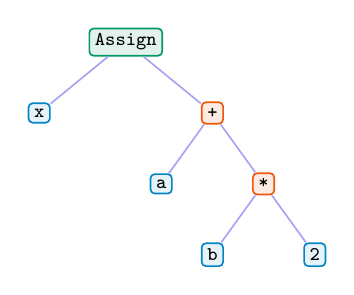
\begin{tikzpicture}[
  level distance=9mm,
  level 1/.style={sibling distance=22mm},
  level 2/.style={sibling distance=13mm},
  every node/.style={draw=ink, rounded corners=1.5pt, fill=card, font=\scriptsize\ttfamily, inner sep=2pt, line width=0.6pt},
  st/.style={draw=emerald, fill=emerald!12},
  ex/.style={draw=orangeC, fill=orangeC!12},
  lf/.style={draw=sky, fill=sky!10},
  edge from parent/.style={draw=indigo!50, line width=0.6pt}]
  \node[st] (as) {Assign}
    child {node[lf] (x) {x}}
    child {node[ex] (pl) {+}
      child {node[lf] (a) {a}}
      child {node[ex] (mu) {*}
        child {node[lf] (b) {b}}
        child {node[lf] (two) {2}}}};
\end{tikzpicture}
\begin{tikzpicture}[overlay, remember picture]\end{tikzpicture}
\vspace{1mm}

\footnotesize
\begin{tabular}{@{}ll@{}}
\toprule
Attribute & Flow on \tm{x = a + b * 2;} \\
\midrule
$\Gamma$ (inherited) & passed down to every leaf; resolves \tm{x}, \tm{a}, \tm{b} \\
$\tau$ (synthesised) & leaves \tm{int}; \tm{*}, \tm{+} give \tm{int}; Assign checks \\
$\mathit{in}$ (inherited) & builds \tm{a + (b*2)} left-associatively \\
unique name & \tm{x}, \tm{a}, \tm{b}; a second \tm{i} becomes \tm{i\#1} \\
\bottomrule
\end{tabular}
\caption{Attributed AST of a simple assignment, coloured as in the GUI:
statements green, expressions orange, leaves blue. The environment flows
down, types flow up, and each identifier is bound to a unique IR name.}
\label{fig:ast}
\end{figure}

\subsection{Three-address code and control flow}

The AST is lowered by a syntax-directed translation into three-address
code whose instructions have the forms $x=y\ \mathit{op}\ z$,
$x=\mathit{op}\ y$, $x=y$, $x=a[i]$, $a[i]=y$, \tm{goto} $L$,
\tm{if} $x$ \tm{goto} $L_t$ \tm{else} $L_f$, \tm{param}, \tm{call},
\tm{return}, \tm{print} and \tm{input}. Conditions are translated as
jumping code~\cite{aho2006dragon}: with true and false targets $t,f$,
\begin{equation}
\begin{aligned}
\mathcal{J}\llbracket B_1 \,\tm{\&\&}\, B_2\rrbracket(t,f) &=
 \mathcal{J}\llbracket B_1\rrbracket(L,f)\ ;\ L{:}\ \mathcal{J}\llbracket B_2\rrbracket(t,f),\\
\mathcal{J}\llbracket B_1 \,\tm{||}\, B_2\rrbracket(t,f) &=
 \mathcal{J}\llbracket B_1\rrbracket(t,L)\ ;\ L{:}\ \mathcal{J}\llbracket B_2\rrbracket(t,f),\\
\mathcal{J}\llbracket \tm{!}B\rrbracket(t,f) &= \mathcal{J}\llbracket B\rrbracket(f,t),
\end{aligned}
\label{eq:jump}
\end{equation}
with $L$ a fresh label, so short-circuit evaluation is exact and no
Boolean value is materialised unless it is stored. Basic blocks are
maximal sequences with a single entry and a single exit. The CFG is
cleaned of unreachable blocks and its critical edges are split, so that
copies inserted later on an edge have a block of their own. Dominators
are computed by the Cooper--Harvey--Kennedy iterative algorithm over
reverse postorder~\cite{cooper2001dom}, natural loops are identified
from back edges $n\to h$ with $h \operatorname{dom} n$, and each block
gets a loop depth. Fig.~\ref{fig:tac} shows the TAC and optimised SSA
the compiler produces for a small loop.

\begin{figure}[t]
\centering
\begin{minipage}[t]{0.47\columnwidth}
\scriptsize\textbf{TAC}\vspace{-1mm}
\begin{verbatim}
entry: n = input()
       s = 0
       i = 0
for1:  t2 = i < n
       if t2 goto body2
             else endfor4
body2: t3 = i % 3
       t4 = t3 == 0
       if t4 goto and7
             else endif6
and7:  t5 = i > 0
       if t5 goto then5
             else endif6
then5: s = s + i
endif6:
step3: i = i + 1
       goto for1
endfor4:
       print s
       return 0
\end{verbatim}
\end{minipage}\hfill
\begin{minipage}[t]{0.5\columnwidth}
\scriptsize\textbf{Optimised SSA}\vspace{-1mm}
\begin{verbatim}
entry: n = input()
       goto for1
for1:  i.2 = phi(0, i.3)
       s.2 = phi(0, s.4)
       if i.2 < n goto body2
             else endfor4
body2: t3 = i.2 % 3
       if t3 == 0 goto and7
             else endif6
and7:  if i.2 > 0 goto then5
             else endif6
then5: s.3 = s.2 + i.2
endif6:
       s.4 = phi(s.2, s.2, s.3)
       i.3 = i.2 + 1
       goto for1
endfor4:
       print s.2
       return 0
\end{verbatim}
\end{minipage}
\caption{Compiler output for
\tm{for(i=0;i<n;i++) if(i\%3==0 \&\& i>0) s+=i;}. Jumping code realises
\tm{\&\&}; after SSA and optimisation, comparisons are fused into
branches and constants into $\varphi$ arguments (split critical-edge
blocks omitted).}
\label{fig:tac}
\end{figure}

\subsection{SSA construction and optimisation}

Liveness is the least fixpoint of
\begin{equation}
\begin{aligned}
\mathit{LiveIn}(b)&=\mathit{use}(b)\cup\big(\mathit{LiveOut}(b)\setminus\mathit{def}(b)\big),\\
\mathit{LiveOut}(b)&=\textstyle\bigcup_{s\in\mathit{succ}(b)}\mathit{LiveIn}(s),
\end{aligned}
\label{eq:liveness}
\end{equation}
solved by a worklist over reverse postorder, with $\varphi$-uses
attributed to the corresponding predecessor edge. SSA is built by the
method of Cytron et~al.~\cite{cytron1991ssa}: for each variable $x$ with
definition blocks $D_x$, a $\varphi$ is placed at every block of the
iterated dominance frontier $\mathit{DF}^{+}(D_x)$ at which $x$ is live
on entry (pruned SSA), and variables are renamed by a walk of the
dominator tree. A read with no reaching definition becomes the
constant~0, which matches MiniC's zero-initialisation of locals.

The optimiser iterates, to a fixpoint or ten rounds, sparse conditional
constant propagation over the lattice
$\top \sqsupset c \sqsupset \bot$ with executable-edge tracking
(SCCP)~\cite{wegman1991sccp}, copy propagation, algebraic simplification
and strength reduction (for example $x\cdot 2^m\Rightarrow x\ll m$,
$x+0\Rightarrow x$), global value numbering scoped by the dominator
tree, dead-code elimination over SSA def-use chains and the merging of
straight-line blocks. It then splits critical edges again and fuses
each comparison with the branch that consumes it into a compare-branch
instruction. Semantic preservation is checked on every benchmark by
executing the SSA program before and after optimisation and comparing
outputs.

\subsection{Profiling and transition probabilities}

The optimised SSA program is executed by a reference interpreter with
bounds-checked memory on a training input. The interpreter counts every
CFG edge $n(b,s)$, and the profiled transition matrix is
\begin{equation}
P_{\mathrm{prof}}(b,s)=\frac{n(b,s)}{\sum_{s'\in\mathit{succ}(b)} n(b,s')},
\label{eq:pprof}
\end{equation}
falling back to the static prior for blocks never reached in training.
The Static-Prior variant uses the classical loop heuristic~\cite{wu1994}
instead: if exactly one successor leaves a loop containing $b$,
\begin{equation}
P_{\mathrm{stat}}(b,s)=\begin{cases}
0.1 & s \text{ exits the loop},\\
0.9 & \text{otherwise},
\end{cases}
\label{eq:pstat}
\end{equation}
and otherwise $P_{\mathrm{stat}}(b,s)=1/|\mathit{succ}(b)|$.
Fig.~\ref{fig:cfg} contrasts the two on the inner loop of the
rare-branch benchmark, where an error path is taken in about 1\% of
iterations but the static prior sees a fair coin.

\begin{figure}[t]
\centering
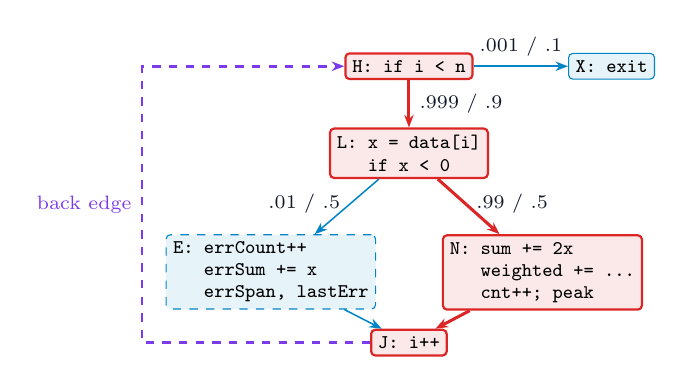
\begin{tikzpicture}[node distance=6mm and 7mm, font=\scriptsize]
  \node[blk, draw=redC, fill=redC!10, line width=0.8pt] (h) {H: if i < n};
  \node[blk, below=of h, draw=redC, fill=redC!10, line width=0.8pt] (l) {L: x = data[i]\\\ \ \ if x < 0};
  \node[blk, below left=7mm and -6mm of l, draw=sky, fill=sky!10, dashed] (e) {E: errCount++\\\ \ \ errSum += x\\\ \ \ errSpan, lastErr};
  \node[blk, below right=7mm and -6mm of l, draw=redC, fill=redC!10, line width=0.8pt] (n) {N: sum += 2x\\\ \ \ weighted += ...\\\ \ \ cnt++; peak};
  \node[blk, below=19mm of l, draw=redC, fill=redC!10, line width=0.8pt] (j) {J: i++};
  \node[blk, right=12mm of h, draw=sky, fill=sky!10] (x) {X: exit};
  \draw[flow, draw=redC, line width=1.1pt] (h) -- node[right,align=left,text=ink]{.999 / .9} (l);
  \draw[flow, draw=sky] (h) -- node[above,text=ink]{.001 / .1} (x);
  \draw[flow, draw=sky] (l) -- node[left, pos=0.45,text=ink]{.01 / .5} (e);
  \draw[flow, draw=redC, line width=1.1pt] (l) -- node[right, pos=0.45,text=ink]{.99 / .5} (n);
  \draw[flow, draw=sky] (e) -- (j);
  \draw[flow, draw=redC, line width=1.1pt] (n) -- (j);
  \draw[flow, draw=violet, dashed, line width=1pt] (j.west) -- ($(j.west -| e.west)+(-3mm,0)$) |- node[pos=0.25,left,text=violet]{back edge} (h.west);
\end{tikzpicture}
\caption{Inner loop of the rare-branch benchmark. Edge labels give
$P_{\mathrm{prof}}/P_{\mathrm{stat}}$. Red marks the hot path found by
profiling and blue the rarely executed blocks: the error block E runs in
1\% of iterations, whereas the static prior assumes 50\%.}
\label{fig:cfg}
\end{figure}

\subsection{The residency MDP of a value}

\begin{definition}[Residency MDP]
For an SSA value $v$ with live range $L_v\subseteq B$, the residency MDP
has states $(b,s)$ with $b\in L_v$ and $s\in\{\Reg,\Mem\}$ (control is in
block $b$ and $v$ is in a register or in its slot). In state $\Reg$ the
actions are \emph{stay} and \emph{spill} (cost $\cst$); in state $\Mem$
they are \emph{stay} and \emph{reload} (cost $\cld$). Control moves from
$b$ to $b'\in L_v$ with probability $P(b,b')$ when $v\in\mathit{LiveIn}(b')$;
leaving the live range is absorbing with value $0$.
\end{definition}

Let $u_v(b)$, $d_v(b)$ and $f_v(b)$ be the numbers of uses,
definitions and \emph{forwardable} uses (a use immediately after the
definition, which the peephole pass turns into a register move when $v$
is spilled) of $v$ in $b$, and $c_v(b)$ the number of calls in $b$
across which $v$ is live. The per-block rewards are
\begin{equation}
\begin{aligned}
r_\Reg(b) &= \csv\,\big(u_v(b)+d_v(b)+f_v(b)\big)-c_v(b)\,(\cst+\cld),\\
r_\Mem(b) &= -\big(u_v(b)\,\cld + d_v(b)\,\cst + f_v(b)\,\cmv\big),
\end{aligned}
\label{eq:reward}
\end{equation}
with $\csv$ a small bonus for a register access, $\cmv$ the cost of a
forwarded move and an extra $-\cld$ in the definition block of a
parameter, which arrives in its slot. The constants are taken from the
simulator's latency table rather than tuned: $\cld$ and $\cst$ are the
load and store latencies, $\cmv=1$ is the latency of the register move
that replaces a forwarded load, and $\csv=1$, one cycle per access,
is the unit of the latency table. $\csv$ is not a physical cost: it
keeps the gain of an accessed value strictly positive and ranks values
with equal spill traffic by how often they are accessed.
Section~\ref{sec:robust} shows that the results change by at most
0.4\% when $\csv$ and $\cmv$ are varied over $\{0,0.5,1,2\}$ and
$\{0,1,2\}$. The optimal values satisfy the
Bellman equations~\cite{bellman1957,puterman1994}
\begin{equation}
\begin{aligned}
V(b,\Reg) &= r_\Reg(b) + \max\big\{\bar V_\Reg(b),\ -\cst + \bar V_\Mem(b)\big\},\\
V(b,\Mem) &= r_\Mem(b) + \max\big\{\bar V_\Mem(b),\ -\cld + \bar V_\Reg(b)\big\},\\
\bar V_s(b) &= \textstyle\sum_{b'\in L_v} P(b,b')\,V(b',s),
\end{aligned}
\label{eq:bellman}
\end{equation}
Fig.~\ref{fig:mdp} draws the two states. Because a live range is left
with probability one under every policy of a terminating program, the
chain restricted to $L_v$ is transient and (\ref{eq:bellman}) is solved
undiscounted, as a total-reward MDP. For a fixed policy $\pi$, policy
evaluation is the sparse linear system
\begin{equation}
\big(I-P_\pi\big)\,V_\pi = r_\pi ,
\label{eq:policyeval}
\end{equation}
where $P_\pi$ is substochastic and transient, so $I-P_\pi$ is a
non-singular M-matrix and Gaussian elimination without pivoting is
stable. Howard's policy iteration~\cite{howard1960} alternates
(\ref{eq:policyeval}) with greedy improvement and terminates in a finite
number of rounds with the exact optimum; we keep value iteration as an
independent cross-check in the test suite. If the restricted chain
were ever not transient, the solver would fall back to a discount factor
$\gamma=0.999$.

\textit{Complexity of Algorithm~\ref{alg:gains}.} The block frequencies
(\ref{eq:freq}) need one sparse solve over the $|B|$ blocks, $O(|B|^3)$
in the worst case for Gaussian elimination. For a value $v$, every
policy-iteration round solves (\ref{eq:policyeval}), a system of
$2|L_v|$ unknowns, which costs $O(|L_v|^3)$ in the worst case and
$O(|L_v|\,w^2)$ when the system, ordered by reverse postorder, has
bandwidth $w$; the improvement step is $O(|L_v|)$. With $R_v$ rounds
and the two forced-policy evaluations, the gains cost
$O\big(|B|^3+\sum_{v}(R_v+2)\,|L_v|^3\big)$ in the worst case. Howard's
method needs few rounds in practice (1.3 on average and at most 7 in
our suites), and coalitions are a union-find pass over the
$\varphi$-edges. The MCS order is $O(|V|+|A|)$, each auction round sorts
at most $k+1$ bids, and binding is $O(|V|\,k+|A|)$; best response
makes at most $2|V|$ moves, each checked in $O(|A|)$, so the auction
and equilibrium steps are dominated by the gains.
Section~\ref{sec:cost} measures how the allocation time grows with
function size and live-range length.

\begin{figure}[t]
\centering
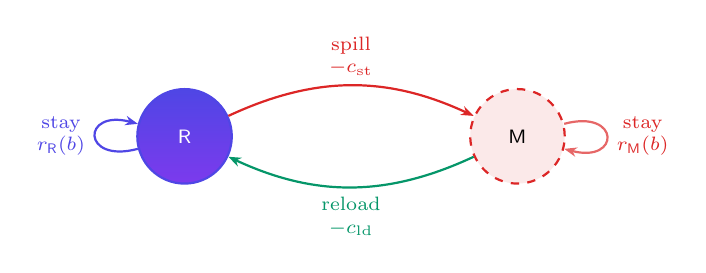
\begin{tikzpicture}[font=\scriptsize, >=Stealth]
  \node[circle, draw=indigo, top color=indigo, bottom color=violet, text=white, minimum size=12mm, line width=0.8pt] (r) {$\Reg$};
  \node[circle, draw=redC, fill=redC!10, minimum size=12mm, line width=0.8pt, dashed, right=30mm of r] (m) {$\Mem$};
  \draw[flow, draw=redC, line width=0.8pt] (r) to[bend left=25] node[above,align=center,text=redC]{spill\\$-\cst$} (m);
  \draw[flow, draw=emerald, line width=0.8pt] (m) to[bend left=25] node[below,align=center,text=emerald]{reload\\$-\cld$} (r);
  \draw[flow, draw=indigo, line width=0.8pt] (r) to[loop left, looseness=6] node[left,align=center,text=indigo]{stay\\$r_\Reg(b)$} (r);
  \draw[flow, draw=redC!70, line width=0.8pt] (m) to[loop right, looseness=6] node[right,align=center,text=redC]{stay\\$r_\Mem(b)$} (m);
\end{tikzpicture}
\caption{The two-state residency MDP replicated over each block $b$ of a
value's live range. In either state control moves to $b'$ with
probability $P(b,b')$; leaving $L_v$ is absorbing with value 0.
Rewards follow (\ref{eq:reward}).}
\label{fig:mdp}
\end{figure}

\subsection{Expected gain of a value}

Neither outcome of the auction leaves the value free to choose its
policy. A loser is forced to stay in $\Mem$ throughout; let
$V_{\mathrm{mem}}$ be the value of that policy, obtained from
(\ref{eq:policyeval}) with $\pi\equiv$ \emph{stay}. A winner is forced
to stay in $\Reg$ throughout, because the code generator does not split
live ranges (Section~\ref{sec:backend}); let $V_{\mathrm{reg}}$ be the
value of that policy, again from (\ref{eq:policyeval}) with
$\pi\equiv$ \emph{stay}. The per-entry gain is the difference between
the two policies that can actually be realised,
$g(v)=V_{\mathrm{reg}}(\mathit{def}(v),\Reg)-V_{\mathrm{mem}}(\mathit{def}(v),\Mem)$.
The optimal value $V^\ast$ of (\ref{eq:bellman}) is still computed: it
bounds the realised gain from above, since always staying in $\Reg$ is
one admissible policy, it shows in the GUI where a value would rather
be spilled or reloaded, and it is the quantity a live-range-splitting
code generator would use. The first draft of this paper bid
$V^\ast(\mathit{def}(v),\Reg)-V_{\mathrm{mem}}$, which values a policy
that is never carried out; Section~\ref{sec:robust} shows that on our
suites the two bids differ by 0.05\% in total and give identical cycle
counts in 48 of 51 configurations.
The live range is entered once for each execution of the definition
block, whose expected count per invocation $\phi$ solves the
Markov-chain flow equations
\begin{equation}
\phi = e_{b_0} + P^{\top}\phi ,
\label{eq:freq}
\end{equation}
so the expected register-residency gain of $v$ per invocation is
\begin{equation}
G(v)=\phi\big(\mathit{def}(v)\big)\cdot
\Big(V_{\mathrm{reg}}\big(\mathit{def}(v),\Reg\big)-V_{\mathrm{mem}}\big(\mathit{def}(v),\Mem\big)\Big).
\label{eq:gain}
\end{equation}
Measuring against $V_{\mathrm{mem}}$ rather than against
$V^\ast(\cdot,\Mem)$ matters: an optimal policy that starts in $\Mem$
may reload at once, which would cap every gain at roughly $\cld$ and
hide the difference between hot and cold values.
$G(v)$ is the quantity a compiler engineer would ask for (expected
cycles saved), and the GUI shows it for every value. In the rare-branch
example of Fig.~\ref{fig:cfg}, the profiled MDP rates the hot-path
accumulators \tm{cnt.3} and \tm{weighted.3} at $G=20{,}300$ and the
error-path counters \tm{errSum.3} and \tm{errCount.3} at $G=180$, a
factor of 113. Under the static prior (\ref{eq:pstat}) all four receive
the same gain, 202.5, because the two arms of the branch look alike;
Static-Prior consequently keeps the error-path value \tm{lastErr} in a
register and spills \tm{cnt} and \tm{weighted}, whereas \MG\ does the
opposite.

\subsection{Coalitions on $\varphi$-webs}

A loop-carried variable is a chain of SSA values joined by
$\varphi$-functions. If they are allocated independently, the auction
may grant a register to one version and not the next, and every
traversal of the back edge then pays a copy through memory. We
therefore form coalitions by union-find over $\varphi$ edges, merging
the argument $a$ and result $p$ of a $\varphi$ in block $h$ along edge
$(b,h)$ only when the edge is \emph{hot}:
\begin{equation}
\phi(b)\,P(b,h) \;\ge\; \theta\cdot\max\big\{\phi(\mathit{def}(a)),\ \phi(h)\big\},
\qquad \theta=0.75 .
\label{eq:hot}
\end{equation}
A loop-carried variable thus forms one coalition around its back edge,
while a copy made once on loop entry, or on a rare path, does not drag
a cold value into a hot coalition. The threshold $\theta$ was chosen on
a separate tuning suite of five programs that is not used in any
reported result (Section~\ref{sec:params}). Every member of coalition $C$ bids the
coalition's total gain,
\begin{equation}
\beta(v)=\sum_{w\in C(v)} G(w),
\label{eq:bid}
\end{equation}
so the coalition wins or loses as a unit. This is the transferable-utility
view of cooperative game theory~\cite{shapley1953}: the coalition's
value is what its members achieve together, and (\ref{eq:bid}) lets
members with small individual gains (for example the version of
\tm{i} after the increment, $G=12{,}288$) inherit the bid of the whole
web ($\beta=94{,}223$).

\subsection{Sealed-bid auction on the chordal interference graph}

The interference graph $\mathcal{I}=(V,A)$ joins two values when one is
live at the definition of the other. On strict SSA $\mathcal{I}$ is
chordal~\cite{hack2006ssa}; we compute a maximum cardinality search
order $\sigma$~\cite{tarjan1984} and verify on every function that its
reverse is a perfect elimination ordering (PEO), which held for all
functions in our suite. In a chordal graph visited in MCS order, the
already-visited neighbours of each vertex form a clique, so when $v$
arrives its already-visited neighbours together with $v$ are a clique
$Q_v$, a set of values that are all simultaneously live.

The auction (Algorithm~\ref{alg:auction}) visits values in order
$\sigma$. If $v$ has fewer than $k$ already-winning neighbours, it wins
outright. Otherwise $Q_v$ exceeds the register budget and a sealed-bid
round awards the $k$ registers of that clique to the $k$ highest bids:
\begin{equation}
W(Q_v) = \arg\max_{S\subseteq Q_v,\ |S|\le k}\ \sum_{w\in S}\beta(w),
\label{eq:auction}
\end{equation}
which for a single capacity constraint is solved exactly by sorting.
Ties are broken by $\sigma$, so the result is deterministic. Losers are
spilled to slots that are shared by every member of a $\varphi$-web,
so that spilled $\varphi$ copies become no-ops. Registers are then bound
along $\sigma$, choosing for each winner a register not held by any
winning neighbour and preferring one already held by a member of its
web, so the $\varphi$ copy disappears. Fig.~\ref{fig:auction} shows a
real auction round from the rare-branch benchmark at $k=4$.

\begin{figure}[t]
\centering
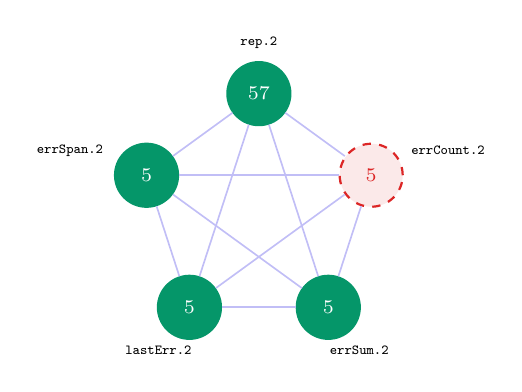
\begin{tikzpicture}[font=\scriptsize]
  \foreach \name/\lab/\bid/\ang/\win in {
      a/rep.2/57/90/1, b/errSpan.2/5/162/1, c/lastErr.2/5/234/1,
      d/errSum.2/5/306/1, e/errCount.2/5/18/0} {
    \ifnum\win=1
      \node[circle, draw=emerald, fill=emerald, text=white, minimum size=8mm, inner sep=0pt, line width=0.8pt]
        (\name) at (\ang:15mm) {\bid};
    \else
      \node[circle, draw=redC, dashed, fill=redC!10, text=redC, minimum size=8mm, inner sep=0pt, line width=0.8pt]
        (\name) at (\ang:15mm) {\bid};
    \fi
    \node[font=\tiny\ttfamily, anchor=\ang+180] at (\ang:19.5mm) {\lab};
  }
  \foreach \u/\v in {a/b,a/c,a/d,a/e,b/c,b/d,b/e,c/d,c/e,d/e}
    \draw[draw=indigo!35, line width=0.6pt] (\u) -- (\v);
\end{tikzpicture}
\caption{An auction round at $k=4$ in the rare-branch benchmark:
when \tm{errCount.2} arrives in MCS order its clique has five members.
Node labels are bids $\beta$; the four highest win (green), and the tie
at 5 is broken by MCS order, so \tm{errCount.2} is spilled (red, dashed).
The GUI uses the same colours for auction winners and losers.}
\label{fig:auction}
\end{figure}

\begin{algorithm}[t]
\caption{Profile-driven gains and coalition bids}
\label{alg:gains}
\begin{algorithmic}[1]
\REQUIRE SSA function with CFG $\mathcal{C}$, edge counts $n$ (or none)
\ENSURE gains $G$, bids $\beta$, coalitions $C$
\STATE $P \leftarrow$ (\ref{eq:pprof}) if $n$ given, else (\ref{eq:pstat})
\STATE $\phi \leftarrow$ solve $(I-P^\top)\phi=e_{b_0}$ \hfill (\ref{eq:freq})
\FORALL{$v\in V$}
  \STATE build rewards $r_\Reg, r_\Mem$ on $L_v$ \hfill (\ref{eq:reward})
  \STATE $\pi \leftarrow$ \emph{stay} in every state
  \REPEAT
    \STATE $V_\pi \leftarrow$ solve $(I-P_\pi)V_\pi=r_\pi$ \hfill (\ref{eq:policyeval})
    \STATE $\pi' \leftarrow$ greedy in (\ref{eq:bellman}) w.r.t.\ $V_\pi$
    \STATE \textbf{if} $\pi'=\pi$ \textbf{then break}; $\pi\leftarrow\pi'$
  \UNTIL{false}
  \STATE $V^\ast\leftarrow V_\pi$ \COMMENT{optimal; kept for display and splitting}
  \STATE $V_{\mathrm{reg}}, V_{\mathrm{mem}} \leftarrow$ evaluate $\pi\equiv$\,\emph{stay} from $\Reg$ and from $\Mem$
  \STATE $g\leftarrow V_{\mathrm{reg}}(\mathit{def}(v),\Reg)-V_{\mathrm{mem}}(\mathit{def}(v),\Mem)$
  \STATE $G(v)\leftarrow \phi(\mathit{def}(v))\cdot g$ \hfill (\ref{eq:gain})
\ENDFOR
\STATE $C \leftarrow$ union-find over $\varphi$ edges satisfying (\ref{eq:hot})
\STATE $\beta(v)\leftarrow\sum_{w\in C(v)}G(w)$ for all $v$ \hfill (\ref{eq:bid})
\RETURN $G,\beta,C$
\end{algorithmic}
\end{algorithm}

\begin{algorithm}[t]
\caption{MCS-ordered sealed-bid auction and register binding}
\label{alg:auction}
\begin{algorithmic}[1]
\REQUIRE interference graph $\mathcal{I}$, bids $\beta$, $k$, webs
\ENSURE allocation $\rho$
\STATE $\sigma\leftarrow$ \textsc{MaximumCardinalitySearch}$(\mathcal{I})$; assert reverse$(\sigma)$ is a PEO
\STATE $\mathit{win}\leftarrow\emptyset$
\FORALL{$v$ in order $\sigma$}
  \STATE $R\leftarrow\{w\in\mathrm{adj}(v)\mid w\in\mathit{win}\}$
  \IF{$|R|<k$}
    \STATE $\mathit{win}\leftarrow\mathit{win}\cup\{v\}$
  \ELSE
    \STATE $Q\leftarrow R\cup\{v\}$ \COMMENT{a clique}
    \STATE $S\leftarrow$ top-$k$ of $Q$ by $(\beta,-\sigma)$ \hfill (\ref{eq:auction})
    \STATE $\mathit{win}\leftarrow(\mathit{win}\setminus Q)\cup S$
  \ENDIF
\ENDFOR
\FORALL{$v\in\mathit{win}$ in order $\sigma$}
  \STATE $F\leftarrow\{0..k{-}1\}\setminus\{\rho(w)\mid w\in\mathrm{adj}(v)\}$
  \STATE $\rho(v)\leftarrow$ a register of $F$ held by $v$'s web, else $\min F$
\ENDFOR
\RETURN $\rho$ (values without a register are spilled)
\end{algorithmic}
\end{algorithm}

\subsection{Best-response dynamics and equilibrium}

The auction decides each clique locally, so a loser can end up with a
register that none of its neighbours actually uses (for example
because a rival that beat it later lost elsewhere). We model the result
as a game whose players are coalitions, whose strategies are a
register for each member or memory, and whose payoff is $\beta$ when
all members hold registers and $0$ otherwise, subject to the
non-interference constraint. A spilled coalition $C$ has a profitable
unilateral deviation if
\begin{equation}
\beta(C)>0\ \wedge\ \forall v\in C:\ \{0,\dots,k{-}1\}\setminus\rho\big(\mathrm{adj}(v)\big)\neq\emptyset .
\label{eq:nash}
\end{equation}
Best-response dynamics (Algorithm~\ref{alg:br}) let deviating
coalitions take free registers, highest bid first, until none can.

Splitting a coalition between registers and memory costs a copy through
memory on each hot $\varphi$ edge that joins a winner and a loser. When
that expected penalty is at least the winners' own gain,
\begin{equation}
\sum_{\substack{(b,h)\ \varphi\text{-edge}\\ \text{split}}}\phi(b)\,P(b,h)\,c_{(b,h)}
\;\ge\;\sum_{w\in C,\ \rho(w)\neq\bot}G(w),
\label{eq:repair}
\end{equation}
with $c_{(b,h)}$ equal to $\cld$ or $\cst$ depending on the direction of
the copy, the winners concede and the whole coalition leaves the
game: it is added to an exclusion set $X$ that every later
best-response pass skips (Algorithm~\ref{alg:br}, lines 1, 6 and 13),
so a conceded coalition can never take registers again. Best response
then runs once more, over the coalitions not in $X$, to reuse the freed
registers.

\begin{proposition}
\label{prop:br}
Algorithm~\ref{alg:br}, including the repair step, terminates after at
most $2|V|$ deviations and $|V|$ concessions, and its result is a pure
Nash equilibrium of the game among the coalitions not in $X$: no
spilled coalition outside $X$ satisfies (\ref{eq:nash}), and no winning
coalition can raise its payoff by deviating.
\end{proposition}
\begin{proofsketch}
Let $\Phi(\rho)$ be the number of values that hold a register. In
\textsc{BestResponse}, a deviation moves a whole coalition from memory
into registers that are free with respect to all of its neighbours,
without evicting anyone, so $\Phi$ grows strictly and is bounded by
$|V|$: the first pass makes at most $|V|$ deviations. The repair step
is a single pass over the coalitions; it only removes values, each
coalition is demoted at most once, and every demoted coalition enters
$X$, so at most $|V|$ values are conceded. The second pass skips $X$,
so it cannot re-admit a conceded coalition and cannot undo the repair;
by the same argument on $\Phi$ it makes at most $|V|$ further
deviations and ends when (\ref{eq:nash}) fails for every spilled
coalition outside $X$. Coalitions in $X$ have conceded because the
copy penalty (\ref{eq:repair}) of a split allocation exceeds their
gain, so they are not players of the final game. A winning coalition
already receives its maximal payoff $\beta(C)$, and changing to
another free register leaves the payoff unchanged, so no player has a
strictly profitable deviation.
\end{proofsketch}

We describe the game cautiously. Because two interfering values may not
share a register, it is not a congestion game in Rosenthal's
sense~\cite{rosenthal1973}: a player's payoff depends on which
neighbours in the interference graph hold which registers, not on how
many players use a resource, which makes it closer to the graph-colouring
games studied by Panagopoulou and Spirakis~\cite{panagopoulou2008}. We
do not claim an exact potential function~\cite{monderer1996} for the
general game, in which players could also switch or evict. For the
restricted dynamics of Algorithm~\ref{alg:br}, which only admit
deviations from memory into free registers, $\Phi$ above is a potential
that increases with every move, which is all that the termination
argument needs. The equilibrium need not maximise
(\ref{eq:objective}) globally, and such games have many equilibria. The
auction is what steers the dynamics towards a high-gain equilibrium:
best response only fills registers that the auction left free.

\begin{algorithm}[t]
\caption{Best-response dynamics with coalition repair}
\label{alg:br}
\begin{algorithmic}[1]
\REQUIRE $\rho$ from Algorithm~\ref{alg:auction}, coalitions $C$, bids $\beta$, gains $G$
\ENSURE equilibrium allocation $\rho$
\STATE $X\leftarrow\emptyset$ \COMMENT{coalitions that have left the game}
\STATE \textsc{BestResponse}$(\rho, X)$
\FORALL{coalitions $C$ split between registers and memory}
  \IF{(\ref{eq:repair}) holds for $C$}
    \STATE $\rho(w)\leftarrow\bot$ for every $w\in C$
    \STATE $X\leftarrow X\cup\{C\}$
  \ENDIF
\ENDFOR
\STATE \textbf{if} $X\neq\emptyset$ \textbf{then} \textsc{BestResponse}$(\rho, X)$
\RETURN $\rho$
\item[]
\item[] \textbf{procedure} \textsc{BestResponse}$(\rho, X)$
\REPEAT
  \STATE $\mathit{changed}\leftarrow$ false
  \FORALL{spilled coalitions $C\notin X$ by decreasing $\beta$}
    \IF{every $v\in C$ has a free register (\ref{eq:nash})}
      \STATE assign them, preferring registers of web partners
      \STATE $\mathit{changed}\leftarrow$ true
    \ENDIF
  \ENDFOR
\UNTIL{not $\mathit{changed}$}
\end{algorithmic}
\end{algorithm}

\begin{figure*}[!t]
\centering
\begin{minipage}[t]{0.40\textwidth}\vspace{0pt}\centering
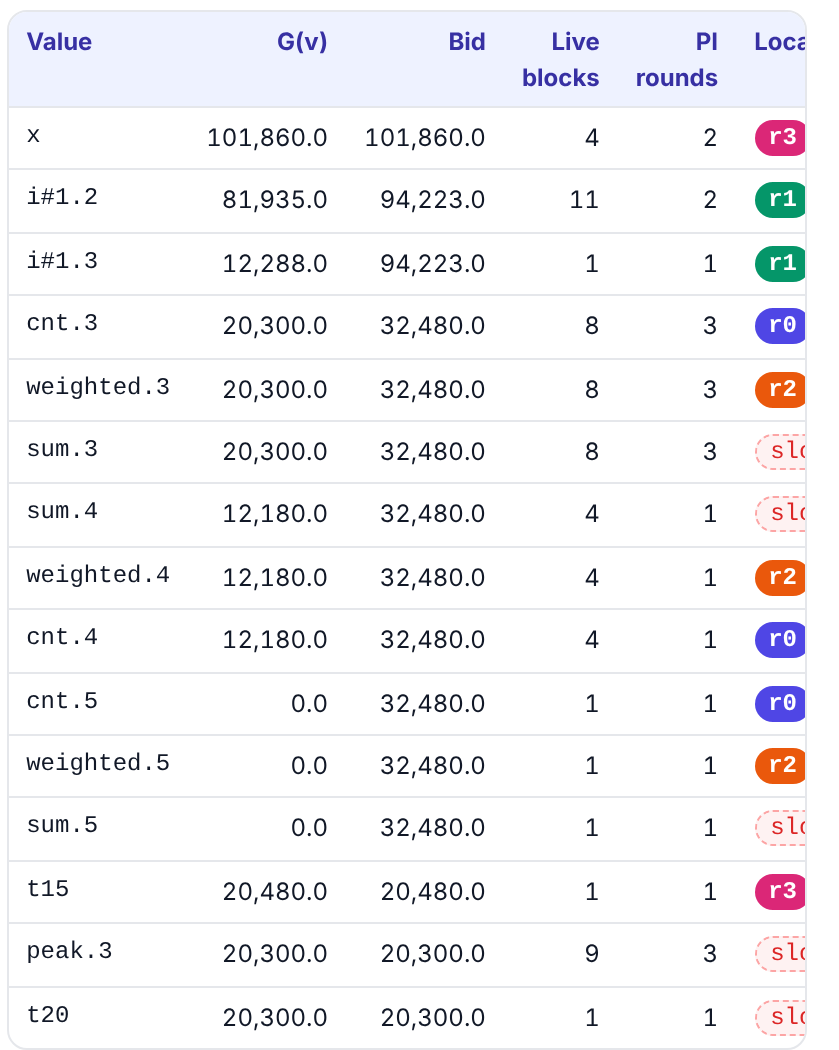
\includegraphics[width=\linewidth]{c_alloc_table.png}\\[-1pt]
{\footnotesize (a) Gains $G(v)$, coalition bids, live-range size, policy-iteration rounds and location}
\end{minipage}\hfill
\begin{minipage}[t]{0.57\textwidth}\vspace{0pt}\centering
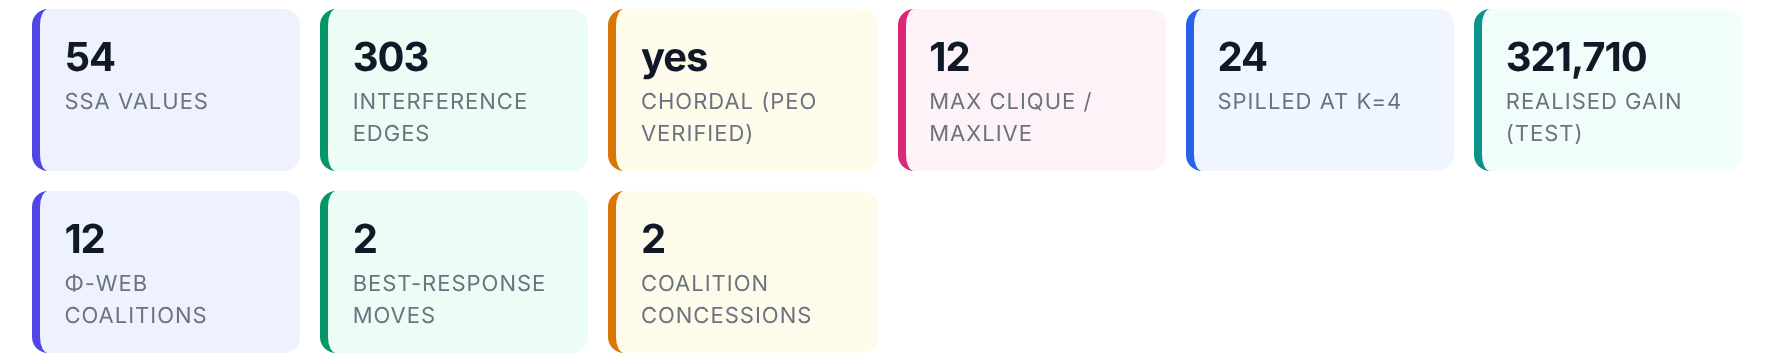
\includegraphics[width=\linewidth]{c_alloc_stats.png}\\[-1pt]
{\footnotesize (b) Summary of the allocation of \tm{main}}\\[6pt]
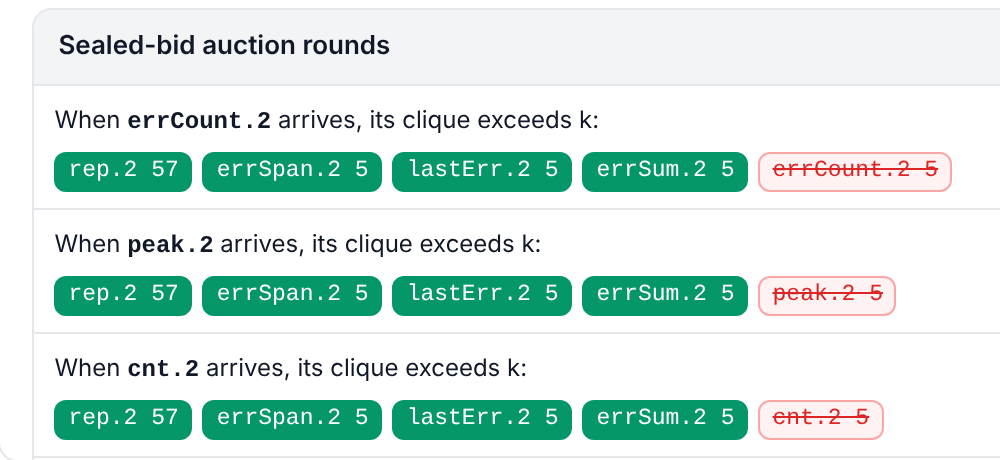
\includegraphics[width=\linewidth]{c_alloc_rounds.png}\\[-1pt]
{\footnotesize (c) The first auction rounds in MCS order: winners in green, losers in red}
\end{minipage}
\caption{The Allocation view of the \MG\ Compiler Studio on the
rare-branch benchmark at $k=4$ (training input \tm{7 10}, test input
\tm{13 10}), cropped to its key panels. The full-window screenshots of
every view are provided as supplementary material in the repository
(\tm{docs/screenshots}).}
\label{fig:gui}
\end{figure*}

\subsection{Back end: leaving SSA and code generation}
\label{sec:backend}

Fig.~\ref{fig:allocflow} summarises the allocation flow and its
hand-off to the back end. The target, PG-RISC, is a load/store RISC with
allocatable registers $r_0,\dots,r_{k-1}$, three scratch registers
$t_0$--$t_2$ for spilled operands, a return-value register and a frame
pointer. The frame holds parameters, spill slots (one per $\varphi$-web),
caller-save slots and local arrays. $\varphi$-functions are replaced by
parallel copies on the (already split) incoming edges, sequentialised
with cycles broken through $t_2$; copies between values that share a
register or a slot vanish. Registers live across a call are saved and
restored around it. A peephole pass threads jumps, removes jumps to the
next instruction and forwards a store to an immediately following load
of the same slot, turning the load into a move or deleting it, which
is the forwarding that $f_v(b)$ in (\ref{eq:reward}) anticipates.

\begin{figure}[t]
\centering
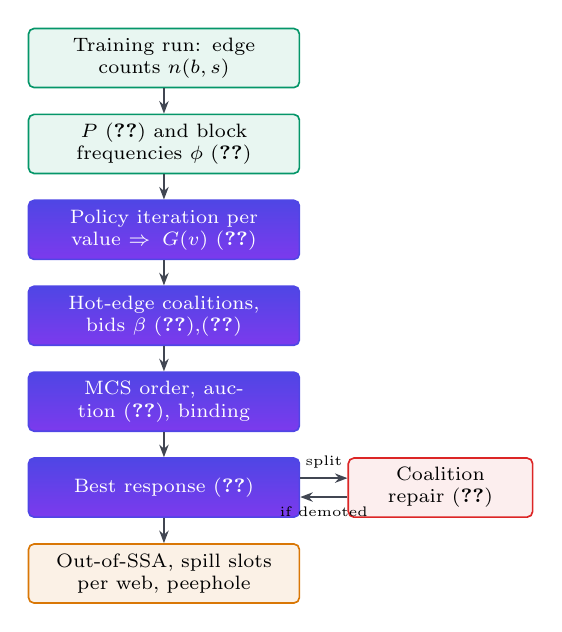
\begin{tikzpicture}[node distance=3.2mm, font=\scriptsize]
  \node[midst, text width=33mm] (a) {Training run: edge counts $n(b,s)$};
  \node[midst, text width=33mm, below=of a] (b) {$P$ (\ref{eq:pprof}) and block frequencies $\phi$ (\ref{eq:freq})};
  \node[hot, text width=33mm, below=of b] (c) {Policy iteration per value $\Rightarrow G(v)$ (\ref{eq:gain})};
  \node[hot, text width=33mm, below=of c] (d) {Hot-edge coalitions, bids $\beta$ (\ref{eq:hot}),(\ref{eq:bid})};
  \node[hot, text width=33mm, below=of d] (e) {MCS order, auction (\ref{eq:auction}), binding};
  \node[hot, text width=33mm, below=of e] (f) {Best response (\ref{eq:nash})};
  \node[back, text width=33mm, below=of f] (g) {Out-of-SSA, spill slots per web, peephole};
  \node[stage, draw=redC, fill=redC!8, text width=22mm, right=6mm of f] (r) {Coalition repair (\ref{eq:repair})};
  \foreach \x/\y in {a/b,b/c,c/d,d/e,e/f,f/g} \draw[flow] (\x) -- (\y);
  \draw[flow] ($(f.east)+(0,1.2mm)$) -- node[above,font=\tiny]{split} ($(r.west)+(0,1.2mm)$);
  \draw[flow] ($(r.west)+(0,-1.2mm)$) -- node[below,font=\tiny]{if demoted} ($(f.east)+(0,-1.2mm)$);
\end{tikzpicture}
\caption{Flow of the \MG\ allocator, from profile to target code.}
\label{fig:allocflow}
\end{figure}

\subsection{Modules and the team's contribution}

The work divides into modules owned by the team members (the full list
is given in the contributions section). The core pipeline
module provides the lexer, the grammar and its LL(1) verification, the
parser and AST, and TAC generation (Shreyans Chowdry). The semantic
module provides the scoped symbol table, the attribute evaluation and
diagnostics (Samrender Singh Saini). The optimisation and code-generation
module provides SSA, the optimiser, the \MG\ gain engine and PG-RISC code
generation (Karthikeya Jami). The runtime and evaluation module provides
the interpreter, the simulator, the test suite and the benchmark
harness (Abhishek Kumar). The web GUI and its visualisations are part of
the core pipeline module (Shreyans Chowdry), with documentation and
interface testing support from Nishanth Kumar. Within the \MG\ allocator
itself, the work is divided among four members: the profile-derived
transition matrices, block frequencies and $\varphi$-web coalitions
(Shreyans Chowdry); the interference graph, MCS order and sealed-bid
auction (Samrender Singh Saini); the residency MDP, policy iteration and
gains (Karthikeya Jami); and best response, coalition repair and the
baselines (Abhishek Kumar).

\begin{figure*}[!t]
\centering
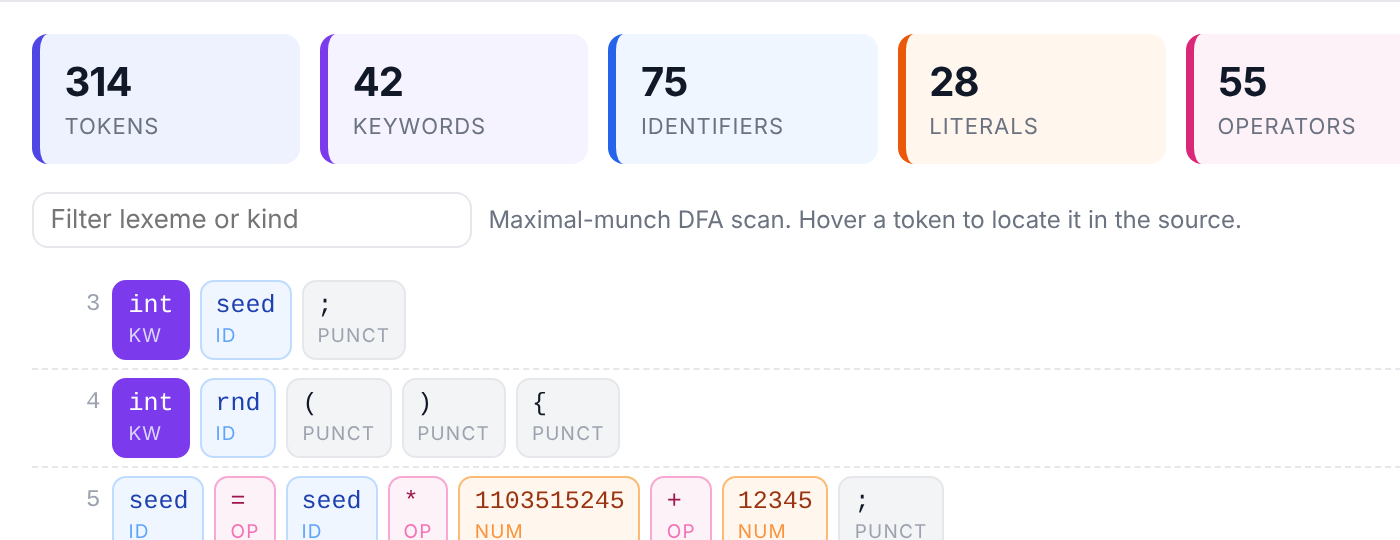
\includegraphics[width=0.80\textwidth]{c_tokens.png}\\[-1pt]
{\footnotesize (a) Tokens view: counts by kind and the token stream of the maximal-munch DFA, coloured by kind}\\[6pt]
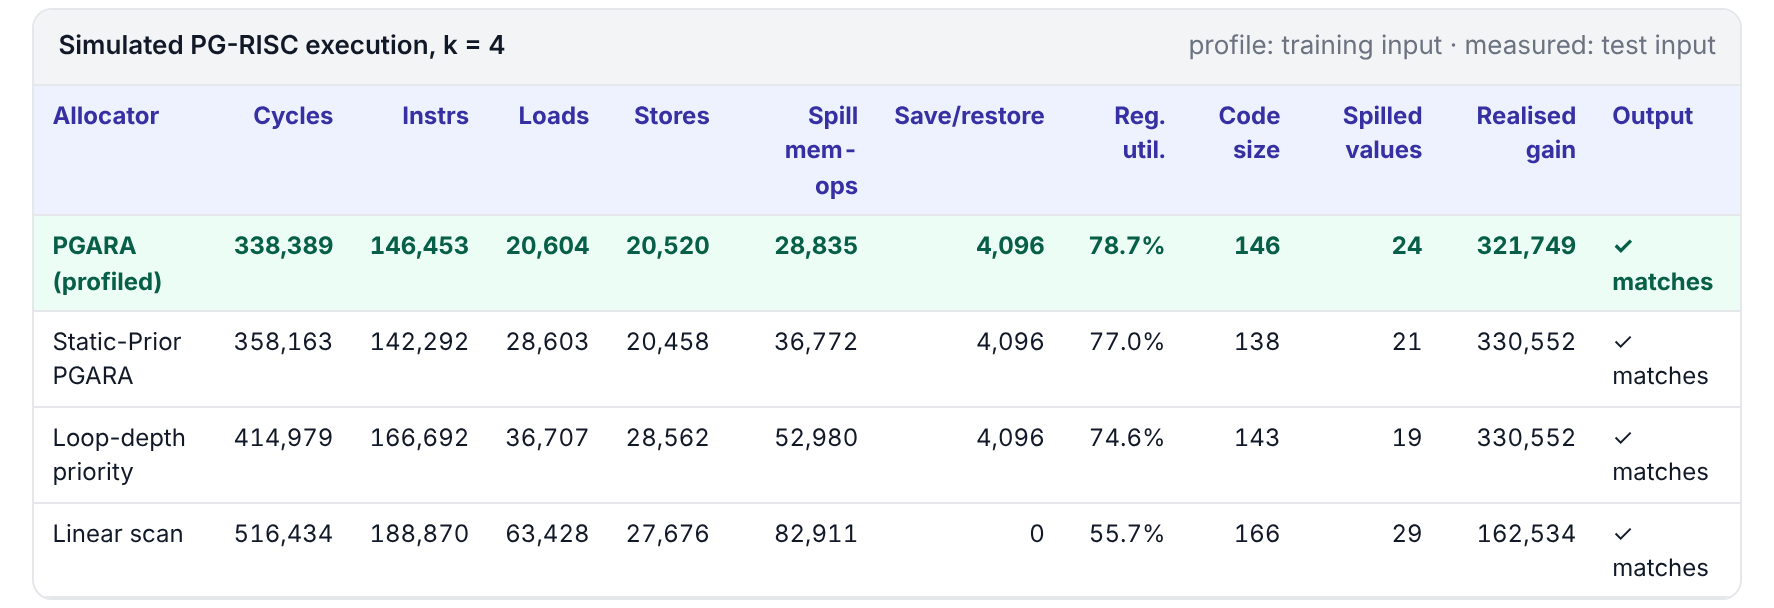
\includegraphics[width=0.80\textwidth]{c_run.png}\\[-1pt]
{\footnotesize (b) Run \& Metrics view: the four allocators of the GUI compared on the test input}
\caption{Two further views of the \MG\ Compiler Studio on the
rare-branch benchmark, cropped so that the text is legible in print.
The AST and CFG views correspond to Figs.~\ref{fig:ast} and~\ref{fig:cfg};
full screenshots of all ten views are in the repository.}
\label{fig:guitabs}
\end{figure*}

%% =====================================================================
\section{Implementation and Result Analysis}
\label{sec:impl}

\subsection{Tools and setup}

The compiler is written in Python~3 using only the standard library, so
it runs on any machine with a recent Python installation and no package
manager~\cite{python}. A small HTTP server from the standard library
serves the web interface and a JSON compilation endpoint; the interface
is plain HTML, CSS and JavaScript with hand-drawn SVG for trees and
graphs, using a colour code that is consistent across views (token
kinds, AST node categories, one colour per register, red for spills,
green for auction winners, and a blue-to-red heat scale for block
frequencies), so that the same colours used in the figures of this
paper appear on screen. The GUI is started with a single start-up
script, which launches the server on port 8765 and opens the browser,
and every experiment in this section is run with one command-line
invocation that writes JSON results.

A \texttt{unittest} suite of 27 tests covers the lexer, grammar, parser,
semantic checks, SSA invariants (single assignment and dominance of
uses), optimiser semantic preservation, chordality, agreement of policy
and value iteration, a hand-computed gain, the bound
$V_{\mathrm{reg}}\le V^\ast$, auction capacity, the Nash property, the
exclusion of conceded coalitions, feasibility of every baseline, and
end-to-end runs of all allocators on both benchmark suites; all tests
pass. Measured with Coverage.py~\cite{coveragepy}, the suite executes
94\% of the statements of the compiler (97\% of the allocator module),
excluding only the experiment scripts. The interface was exercised end to end in headless
Chromium through Playwright~\cite{playwright}, which also produced the
screenshots in Figs.~\ref{fig:gui} and~\ref{fig:guitabs}.

Each program is compiled at the full optimisation level, profiled on a
training input and measured on a different test input, for every
allocator and $k\in\{3,4,5,6,8,16,32\}$. With 17 programs and seven
allocators this gives 833 configurations, and the multiple-input study
adds 595 more. Every simulated run is compared with the reference
interpreter's output and all 1{,}428 match. Experiments ran on a Linux
container with Python~3.13; because the simulator counts cycles
deterministically, the results do not depend on the host.

\subsection{Parameters and benchmarks}
\label{sec:params}

Table~\ref{tab:params} lists the parameters. The cost model matches the
simulator's latencies, so the gains are expressed in the same cycles
that are measured. Register budgets now extend to $k=16$ and $k=32$,
the sizes of realistic RISC register files, to show what happens when
pressure is low.

Programs come from three disjoint sets. The \emph{original suite} of
ten kernels (Table~\ref{tab:bench}, top) spans straight-line code,
regular loops, recursion and programs whose control flow depends on the
data: a rare error branch, an early-exit search, a switch-like dispatch
chain and a token scanner. The \emph{independent suite} of seven
programs (Table~\ref{tab:bench}, bottom) was translated into MiniC from
well-known embedded benchmarks after the original suite was fixed:
CRC-32, bit counting, Dijkstra's shortest paths and quicksort after
MiBench~\cite{guthaus2001mibench}, Levenshtein distance and an FIR
filter after BEEBS~\cite{pallister2013beebs}, and a 0/1 knapsack.
MiniC has no bitwise operators, so shifts and XOR are written
arithmetically. A separate \emph{tuning suite} of five programs (bubble
sort, prime counting, a histogram with outliers, naive string search and
a gcd table) is used only to choose the hot-edge threshold $\theta$ and
appears in no other result. On the tuning suite, at
$k\in\{3,4,6\}$, the geometric mean of \MG's cycles relative to linear
scan is 0.803 for $\theta\in\{0.05,0.1,0.25\}$, 0.782 for $\theta=0.5$,
0.781 for $\theta=0.75$ and 0.850 without coalitions, so $\theta=0.75$
is used throughout. (The first draft used $\theta=0.25$, chosen on the
evaluation suite itself.) Most programs generate their data with a
linear congruential generator seeded from the input, so training and
test inputs exercise the same code with different data; each program
has five test inputs, and the first is used unless stated otherwise.

\begin{table}[t]
\centering
\caption{Parameter setup}
\label{tab:params}
\footnotesize
\begin{tabular}{@{}lr@{}}
\toprule
Parameter & Value \\
\midrule
Register budgets $k$ & 3, 4, 5, 6, 8, 16, 32 \\
Load / store cost $\cld$ / $\cst$ (cycles) & 4 / 2 \\
Register-access bonus $\csv$, forwarded move $\cmv$ & 1 / 1 \\
ALU / MUL / DIV latency & 1 / 3 / 12 \\
Taken / not-taken branch, call / return & 2 / 1, 3 / 3 \\
Discount $\gamma$ & 1 (fallback 0.999) \\
Static loop-stay probability & 0.9 \\
Hot-edge threshold $\theta$ (tuning suite) & 0.75 \\
Gain policy & always-in-register (\ref{eq:gain}) \\
Optimiser rounds (max) & 10 \\
Interpreter / simulator step limits & $2\cdot10^7$ / $8\cdot10^7$ \\
Programs: original / independent / tuning & 10 / 7 / 5 \\
Test inputs per program & 5 (training $\neq$ test) \\
\bottomrule
\end{tabular}
\end{table}

\begin{table}[t]
\centering
\caption{Benchmarks: SSA values, $\varphi$s, largest interference
clique $\omega$, mean and maximum policy-iteration rounds, profiling
time (interpreter on the training input) and \MG\ allocation time
($k=4$). Top: original suite; bottom: independent suite}
\label{tab:bench}
\footnotesize
\setlength{\tabcolsep}{3.2pt}
\begin{tabular}{@{}lrrrrrrr@{}}
\toprule
Benchmark & $|V|$ & $\varphi$ & $\omega$ & PI$_{\text{mean}}$ & PI$_{\max}$ & prof.\,ms & alloc.\,ms \\
\midrule
straightline & 39 & 0 & 11 & 1.00 & 1 & 0 & 1.2 \\
arraysum & 38 & 16 & 9 & 1.29 & 3 & 67 & 2.9 \\
matmul & 51 & 10 & 8 & 1.27 & 3 & 116 & 2.9 \\
recursion & 39 & 4 & 7 & 1.28 & 3 & 22 & 2.3 \\
rarebranch & 62 & 30 & 12 & 1.26 & 3 & 73 & 9.2 \\
earlyexit & 41 & 17 & 10 & 1.29 & 3 & 112 & 4.1 \\
dispatch & 116 & 55 & 15 & 1.17 & 7 & 45 & 16.2 \\
scanner & 89 & 49 & 11 & 1.15 & 4 & 88 & 11.3 \\
sort & 53 & 16 & 10 & 1.32 & 3 & 211 & 4.4 \\
collatz & 30 & 16 & 9 & 1.53 & 3 & 181 & 5.6 \\
\midrule
crc & 50 & 20 & 13 & 1.38 & 6 & 506 & 7.2 \\
bitcount & 52 & 18 & 10 & 1.44 & 11 & 114 & 8.6 \\
dijkstra & 61 & 19 & 11 & 1.41 & 6 & 469 & 10.5 \\
levenshtein & 65 & 16 & 14 & 1.29 & 6 & 723 & 18.9 \\
knapsack & 48 & 8 & 8 & 1.15 & 2 & 342 & 2.9 \\
fir & 60 & 21 & 11 & 1.23 & 3 & 354 & 5.3 \\
qsort & 72 & 15 & 8 & 1.57 & 10 & 48 & 14.6 \\
\bottomrule
\end{tabular}
\end{table}

\subsection{Baselines and metrics}

We compare seven allocators that share the front end, optimiser,
interference graph and code generator, so that only the allocation
decision differs:
(i)~\MG\ (PG) with profiled probabilities;
(ii)~\emph{Static-Prior} \MG\ (SP), the same engine with (\ref{eq:pstat});
(iii)~\emph{Profiled-frequency priority} (FP), an ablation that keeps
\MG's coalitions, auction, binding and best response but replaces the
MDP gain by the access count weighted by the profiled block frequency
$\phi$ of (\ref{eq:freq}), i.e.\ the 10$^{\text{depth}}$ weight of
(iv) replaced by measured frequency;
(iv)~\emph{Loop-depth priority} (LD), in the style of Chow and
Hennessy~\cite{chow1990}, which weights each access by $10^{\text{depth}}$
and runs the same auction and binding;
(v)~\emph{Chaitin--Briggs with profiled spill costs}
(CBp)~\cite{chaitin1982,briggs1994}: conservative (Briggs) coalescing of
$\varphi$-related values, simplification with optimistic spilling by
lowest cost/degree, and biased colouring towards $\varphi$ partners,
with spill costs (loads, stores and forwarded moves) weighted by the
profiled block frequency, which is how a production allocator uses a
profile~\cite{olesen2011greedy};
(vi)~\emph{Chaitin--Briggs with static costs} (CB), the same with
$10^{\text{depth}}$ weights; and
(vii)~\emph{Linear scan} (LS)~\cite{poletto1999} over live intervals in
layout order, with register hints for $\varphi$ partners.
FP and CBp answer the question whether \MG's gains are worth more than
simply weighting accesses by measured frequency; SP answers whether the
profile is worth anything. PG-RISC is not an LLVM target, so LLVM's own
allocators are represented by these re-implementations rather than run
directly; this keeps every other factor identical.

We report five metrics: (1)~simulated \emph{cycles} on the test input;
(2)~dynamic \emph{spill memory operations}, the loads and stores of
spill slots executed; (3)~\emph{register utilisation},
$1-\text{spill memops}/\text{value accesses}$, the fraction of operand
accesses served from registers; (4)~static \emph{code size} in
instructions; and (5)~\emph{compile cost}, separated into the profiling
run and the allocation itself (Table~\ref{tab:bench} and
Section~\ref{sec:cost}).

\subsection{Execution time}

Table~\ref{tab:k4} lists cycles at $k=4$ for all programs and
allocators, and Fig.~\ref{fig:cycles} shows the four profile-aware or
profile-ablated allocators normalised to linear scan. \MG\ is fastest or
tied on 13 of the 17 programs, and its geometric mean is 21.8\% below
linear scan, 2.6\% below Static-Prior, 3.3\% below profiled-frequency
priority, 3.7\% below Chaitin--Briggs with profiled costs and 5.2\%
below loop-depth priority. The largest gains are on programs with
skewed, data-dependent branches. On rare-branch, \MG\ needs 5.5\% fewer
cycles than Static-Prior, 11.7\% fewer than profiled-frequency priority
and 3.8\% fewer than profiled Chaitin--Briggs, because only the MDP
charges the error-path counters for what they actually cost: the
frequency weight alone still lets the error path's several accesses
add up to a competitive bid. On the independent suite the pattern
repeats: Dijkstra (13\% below FP and 15\% below CBp), knapsack (9\%)
and the FIR filter (2--8\%) favour \MG. \MG\ is not uniformly best.
On quicksort, \MG\ is 4.6\% slower than profiled-frequency priority
and 3.6\% slower than Static-Prior: the recursive partition loop has a phase
behaviour that average-case probabilities blur. On Levenshtein,
loop-depth priority is 0.3\% faster, and Static-Prior is 31\% slower
because the static prior sees the match/mismatch branch as a fair coin.
Straight-line code favours linear scan by 1.4\%: with a single block
there is no uncertainty to exploit.

\begin{table*}[!t]
\centering
\caption{Cycles ($\times10^3$) on the primary test input at $k=4$. Bold: best.
PG: \MG; SP: Static-Prior \MG; FP: profiled-frequency priority; LD:
loop-depth priority; CBp / CB: Chaitin--Briggs with profiled / static
spill costs; LS: linear scan. Top: original suite; bottom: independent
suite}
\label{tab:k4}
\footnotesize
\begin{tabular}{@{}lrrrrrrr@{}}
\toprule
Benchmark & PG & SP & FP & LD & CBp & CB & LS \\
\midrule
straightline & 0.286 & 0.286 & 0.286 & 0.286 & 0.286 & 0.286 & \textbf{0.282} \\
arraysum & \textbf{311.4} & \textbf{311.4} & \textbf{311.4} & \textbf{311.4} & 315.4 & 315.4 & 344.8 \\
matmul & \textbf{565.5} & \textbf{565.5} & \textbf{565.5} & \textbf{565.5} & 583.7 & 583.7 & 817.8 \\
recursion & \textbf{201.6} & \textbf{201.6} & 202.1 & 202.1 & 202.2 & 202.2 & 201.7 \\
rarebranch & \textbf{338.4} & 358.2 & 383.2 & 415.0 & 351.7 & 424.8 & 516.4 \\
earlyexit & 650.6 & \textbf{650.4} & 651.5 & 652.1 & 652.0 & 652.0 & 676.2 \\
dispatch & \textbf{138.8} & \textbf{138.8} & 153.2 & 171.7 & 140.1 & 156.4 & 236.4 \\
scanner & \textbf{411.1} & 479.0 & 431.0 & 480.8 & 474.9 & 516.5 & 530.7 \\
sort & \textbf{849.5} & \textbf{849.5} & 868.8 & 868.8 & 894.4 & 894.4 & 988.4 \\
collatz & \textbf{655.3} & \textbf{655.3} & 657.2 & 657.2 & 657.2 & 657.2 & 942.2 \\
\midrule
crc & \textbf{4009.3} & \textbf{4009.3} & 4026.5 & 4026.5 & 4036.5 & 4036.5 & 4826.2 \\
bitcount & \textbf{629.7} & \textbf{629.7} & 633.2 & 632.9 & 632.1 & 632.1 & 716.8 \\
dijkstra & \textbf{1242.1} & \textbf{1242.1} & 1429.3 & 1474.0 & 1456.3 & 1474.0 & 1661.9 \\
levenshtein & 2721.6 & 3567.6 & 2862.3 & \textbf{2714.2} & 2717.9 & 2717.9 & 3673.8 \\
knapsack & \textbf{734.7} & \textbf{734.7} & 805.1 & 805.1 & 805.2 & 805.2 & 966.5 \\
fir & \textbf{1155.2} & 1167.5 & 1179.7 & 1179.8 & 1249.5 & 1249.5 & 1895.6 \\
qsort & 219.9 & 212.3 & \textbf{210.2} & 223.4 & 222.8 & 219.2 & 293.8 \\
\midrule
geo-mean / LS & 0.782 & 0.803 & 0.808 & 0.825 & 0.812 & 0.830 & 1.000 \\
\bottomrule
\end{tabular}
\end{table*}

\begin{figure*}[!t]
\centering
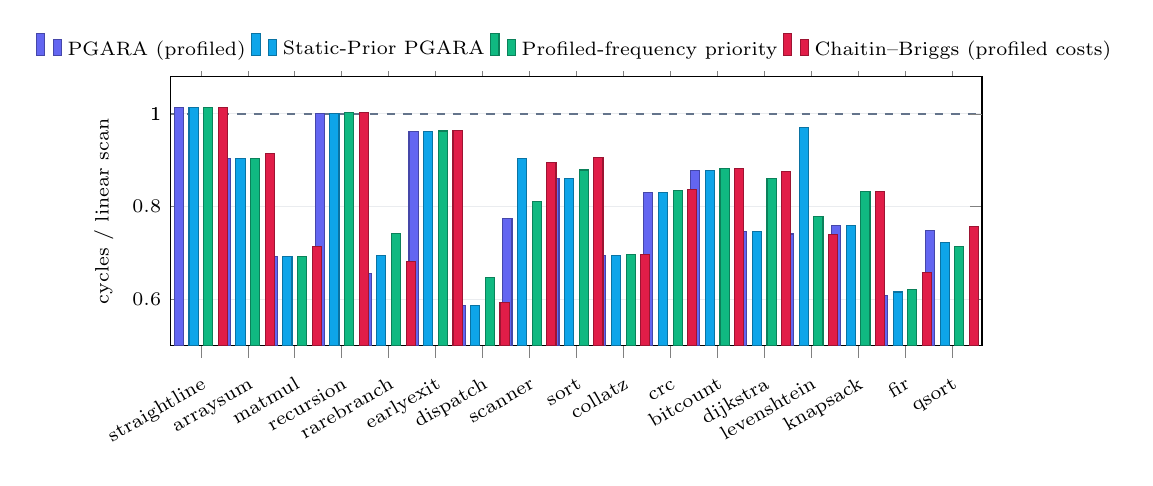
\begin{tikzpicture}
\begin{axis}[
  ybar, bar width=3.3pt, width=0.98\textwidth, height=50mm,
  ymin=0.5, ymax=1.08, ylabel={cycles / linear scan},
  symbolic x coords={straightline,arraysum,matmul,recursion,rarebranch,earlyexit,dispatch,scanner,sort,collatz,crc,bitcount,dijkstra,levenshtein,knapsack,fir,qsort},
  xtick=data, x tick label style={font=\scriptsize, rotate=30, anchor=north east, text height=1.6ex, text depth=0.3ex},
  y tick label style={font=\scriptsize}, ylabel style={font=\scriptsize},
  legend style={font=\scriptsize, at={(0.5,1.02)}, anchor=south, legend columns=4, draw=none},
  ymajorgrids, grid style={draw=rule!80}, enlarge x limits=0.04,
  extra y ticks={1}, extra y tick style={grid=major, grid style={draw=cLS, dashed, line width=0.8pt}},
]
\addplot[fill=cPG, draw=cPG!70!black] coordinates {(straightline,1.014) (arraysum,0.903) (matmul,0.692) (recursion,1.000) (rarebranch,0.655) (earlyexit,0.962) (dispatch,0.587) (scanner,0.775) (sort,0.860) (collatz,0.695) (crc,0.831) (bitcount,0.878) (dijkstra,0.747) (levenshtein,0.741) (knapsack,0.760) (fir,0.609) (qsort,0.748)};
\addplot[fill=cSP, draw=cSP!70!black] coordinates {(straightline,1.014) (arraysum,0.903) (matmul,0.692) (recursion,1.000) (rarebranch,0.694) (earlyexit,0.962) (dispatch,0.587) (scanner,0.903) (sort,0.860) (collatz,0.695) (crc,0.831) (bitcount,0.878) (dijkstra,0.747) (levenshtein,0.971) (knapsack,0.760) (fir,0.616) (qsort,0.722)};
\addplot[fill=cFP, draw=cFP!70!black] coordinates {(straightline,1.014) (arraysum,0.903) (matmul,0.692) (recursion,1.002) (rarebranch,0.742) (earlyexit,0.963) (dispatch,0.648) (scanner,0.812) (sort,0.879) (collatz,0.697) (crc,0.834) (bitcount,0.883) (dijkstra,0.860) (levenshtein,0.779) (knapsack,0.833) (fir,0.622) (qsort,0.715)};
\addplot[fill=cCBp, draw=cCBp!70!black] coordinates {(straightline,1.014) (arraysum,0.915) (matmul,0.714) (recursion,1.003) (rarebranch,0.681) (earlyexit,0.964) (dispatch,0.593) (scanner,0.895) (sort,0.905) (collatz,0.697) (crc,0.836) (bitcount,0.882) (dijkstra,0.876) (levenshtein,0.740) (knapsack,0.833) (fir,0.659) (qsort,0.758)};
\legend{\MG\ (profiled), Static-Prior \MG, Profiled-frequency priority, Chaitin--Briggs (profiled costs)}
\end{axis}
\end{tikzpicture}
\caption{Simulated cycles at $k=4$ on the test inputs, normalised to
linear scan (dashed grey line, 1.0); lower is better. The first ten
programs are the original suite, the last seven the independent suite.
The \MG\ colours match the GUI's Run \& Metrics view.}
\label{fig:cycles}
\end{figure*}

Across register budgets (Table~\ref{tab:gm} and Fig.~\ref{fig:ksweep})
\MG\ has the lowest geometric-mean cycle count at every $k\le 8$:
19--22\% below linear scan, 1.1--3.1\% below Static-Prior, 3.3--4.8\%
below profiled-frequency priority, 1.2--4.5\% below profiled
Chaitin--Briggs and 4.8--6.4\% below loop-depth priority. The advantage
holds on both suites separately: at $k=4$ it is 2.9\% over FP and 2.9\%
over CBp on the original suite, and 3.8\% and 4.9\% on the independent
suite. It is not uniform, however. At $k=3$, profiled Chaitin--Briggs
is 20.7\% faster on matmul and about 12\% faster on Levenshtein and the
FIR filter: under extreme pressure the auction decides each clique
greedily in MCS order and keeps coalitions whole, whereas optimistic
colouring with coalescing finds a tighter packing. These are the cases
where \MG\ is beaten by more than 5\%.

At $k=16$ and $k=32$ register pressure disappears: no auction-based
allocator spills at all, so \MG, Static-Prior and both priority
allocators produce identical code. Chaitin--Briggs is 0.3\% faster
there, because its coalescing removes a few $\varphi$ copies that
\MG's binding hints leave, while \MG\ still needs 16\% and 11\% fewer
cycles than linear scan, which spills at interval boundaries. The benefit of \MG\
therefore lies in the range where registers are scarce, which on real
RISC targets corresponds to code with high register pressure (large
loop bodies, unrolled or inlined code) rather than to typical small
functions. Results are not strictly monotonic in $k$ for every
program, because each extra register that holds a value across a call
adds caller-save traffic.

\begin{table}[t]
\centering
\caption{Geometric-mean cycles over all 17 programs, relative to linear
scan, by register budget. Bold: best}
\label{tab:gm}
\footnotesize
\setlength{\tabcolsep}{3pt}
\begin{tabular}{@{}lrrrrrrr@{}}
\toprule
$k$ & PG & SP & FP & LD & CBp & CB & LS \\
\midrule
3 & \textbf{0.795} & 0.821 & 0.824 & 0.846 & 0.804 & 0.824 & 1.000 \\
4 & \textbf{0.782} & 0.803 & 0.808 & 0.825 & 0.812 & 0.830 & 1.000 \\
5 & \textbf{0.804} & 0.813 & 0.836 & 0.852 & 0.842 & 0.853 & 1.000 \\
6 & \textbf{0.805} & 0.820 & 0.846 & 0.861 & 0.842 & 0.852 & 1.000 \\
8 & \textbf{0.807} & 0.819 & 0.842 & 0.848 & 0.837 & 0.841 & 1.000 \\
16 & 0.843 & 0.843 & 0.843 & 0.843 & \textbf{0.841} & \textbf{0.841} & 1.000 \\
32 & 0.891 & 0.891 & 0.891 & 0.891 & \textbf{0.888} & \textbf{0.888} & 1.000 \\
\bottomrule
\end{tabular}
\end{table}

\begin{figure}[t]
\centering
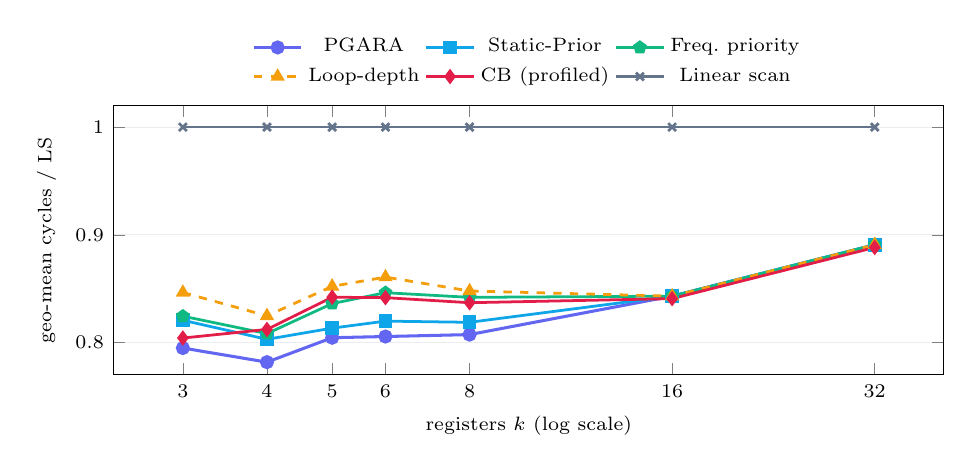
\begin{tikzpicture}
\begin{semilogxaxis}[
  width=\columnwidth, height=50mm, xlabel={registers $k$ (log scale)},
  ylabel={geo-mean cycles / LS}, xtick={3,4,5,6,8,16,32}, xticklabels={3,4,5,6,8,16,32},
  ymin=0.77, ymax=1.02, legend style={font=\scriptsize, at={(0.5,1.03)}, anchor=south, legend columns=3, draw=none},
  tick label style={font=\scriptsize}, label style={font=\scriptsize},
  ymajorgrids, grid style={draw=rule!80}]
\addplot[cPG, mark=*, line width=1.1pt] coordinates {(3,0.7948) (4,0.7817) (5,0.8044) (6,0.8055) (8,0.8073) (16,0.8430) (32,0.8907)};
\addplot[cSP, mark=square*, line width=1pt] coordinates {(3,0.8206) (4,0.8029) (5,0.8133) (6,0.8198) (8,0.8187) (16,0.8430) (32,0.8907)};
\addplot[cFP, mark=pentagon*, line width=1pt] coordinates {(3,0.8244) (4,0.8082) (5,0.8361) (6,0.8462) (8,0.8419) (16,0.8430) (32,0.8907)};
\addplot[cLD, dashed, mark=triangle*, mark options={solid}, line width=1pt] coordinates {(3,0.8464) (4,0.8247) (5,0.8521) (6,0.8607) (8,0.8478) (16,0.8430) (32,0.8907)};
\addplot[cCBp, mark=diamond*, line width=1pt] coordinates {(3,0.8041) (4,0.8121) (5,0.8420) (6,0.8416) (8,0.8369) (16,0.8407) (32,0.8882)};
\addplot[cLS, mark=x, line width=1pt] coordinates {(3,1.0000) (4,1.0000) (5,1.0000) (6,1.0000) (8,1.0000) (16,1.0000) (32,1.0000)};
\legend{\MG, Static-Prior, Freq.\ priority, Loop-depth, CB (profiled), Linear scan}
\end{semilogxaxis}
\end{tikzpicture}
\caption{Geometric-mean cycles over the 17 programs, normalised to
linear scan, as the register budget varies from 3 to 32.}
\label{fig:ksweep}
\end{figure}

\subsection{Spill traffic and register utilisation}

Dynamic spill traffic (Fig.~\ref{fig:spills}) is where the
expected-gain objective shows most directly, because (\ref{eq:gain})
is precisely the expected spill traffic avoided. Summed over the 17
programs at $k=4$, \MG\ executes 50\% fewer spill memory operations than
linear scan, 23\% fewer than Static-Prior, 12\% fewer than
profiled-frequency priority and 15\% fewer than profiled
Chaitin--Briggs; at $k=8$ it nearly eliminates spill traffic (68k
operations against 137k, 205k, 172k and 593k). The exception is again
$k=3$, where profiled Chaitin--Briggs executes 1.5\% fewer spill
operations than \MG. Register utilisation (Fig.~\ref{fig:util})
follows: the mean fraction of operand accesses served from registers
rises from 76\% at $k=3$ to 98\% at $k=8$ for \MG, against 67\% to 91\%
for linear scan, and reaches 100\% for every allocator except linear
scan at $k=16$. The number of \emph{static} spilled values can be
higher for \MG\ than for the priority allocators: \MG\ deliberately
spills many cold values in order to keep the few hot ones, which is the
intended behaviour of a gain-maximising allocator.

\begin{figure}[t]
\centering
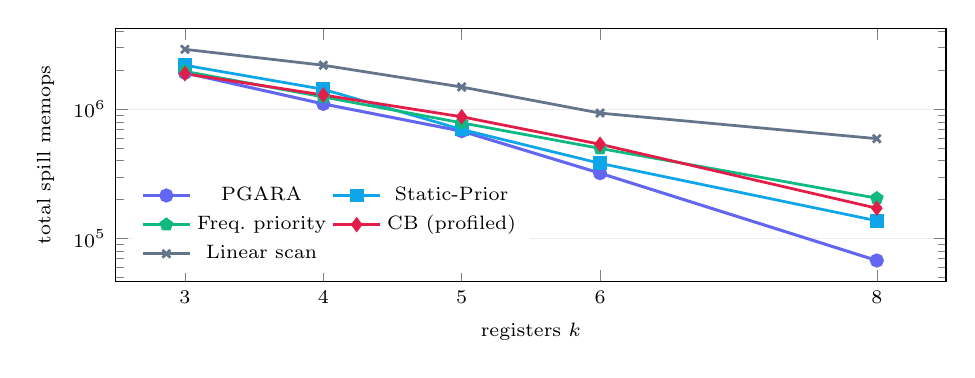
\begin{tikzpicture}
\begin{semilogyaxis}[
  width=\columnwidth, height=48mm, xlabel={registers $k$},
  ylabel={total spill memops}, xtick={3,4,5,6,8},
  legend style={font=\scriptsize, at={(0.02,0.03)}, anchor=south west, draw=none, fill=white, legend columns=2},
  tick label style={font=\scriptsize}, label style={font=\scriptsize},
  ymajorgrids, grid style={draw=rule!80}]
\addplot[cPG, mark=*, line width=1.1pt] coordinates {(3,1915169) (4,1100831) (5,677926) (6,320390) (8,67607)};
\addplot[cSP, mark=square*, line width=1pt] coordinates {(3,2192760) (4,1427803) (5,698680) (6,381852) (8,137323)};
\addplot[cFP, mark=pentagon*, line width=1pt] coordinates {(3,1967620) (4,1246262) (5,785645) (6,498035) (8,205271)};
\addplot[cCBp, mark=diamond*, line width=1pt] coordinates {(3,1887008) (4,1290115) (5,875320) (6,536513) (8,171682)};
\addplot[cLS, mark=x, line width=1pt] coordinates {(3,2911238) (4,2192849) (5,1488122) (6,934693) (8,592789)};
\legend{\MG, Static-Prior, Freq.\ priority, CB (profiled), Linear scan}
\end{semilogyaxis}
\end{tikzpicture}
\caption{Dynamic spill loads and stores summed over the 17 programs
(log scale). At $k\ge16$ only linear scan spills.}
\label{fig:spills}
\end{figure}

\begin{figure}[t]
\centering
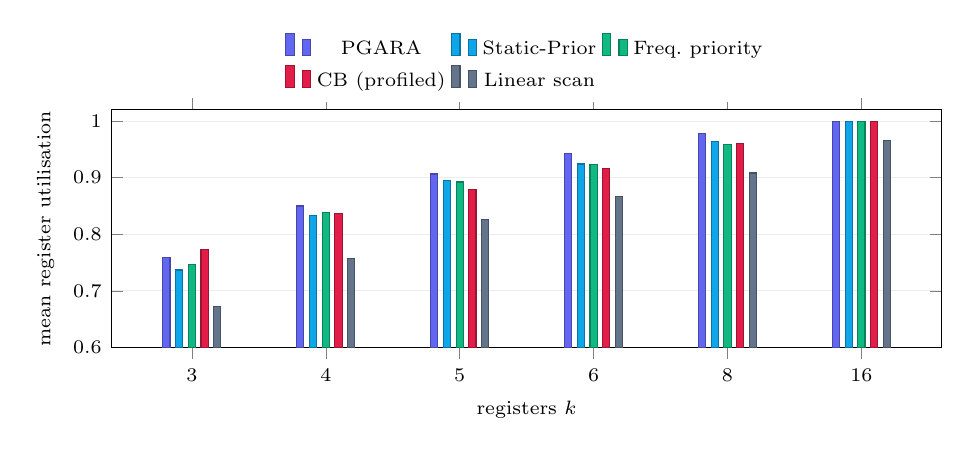
\begin{tikzpicture}
\begin{axis}[
  ybar, bar width=2.6pt, width=\columnwidth, height=46mm,
  xlabel={registers $k$}, ylabel={mean register utilisation},
  symbolic x coords={3,4,5,6,8,16}, xtick=data, ymin=0.6, ymax=1.02,
  legend style={font=\scriptsize, at={(0.5,1.03)}, anchor=south, legend columns=3, draw=none},
  tick label style={font=\scriptsize}, label style={font=\scriptsize},
  ymajorgrids, grid style={draw=rule!80}, enlarge x limits=0.12]
\addplot[fill=cPG, draw=cPG!70!black] coordinates {(3,0.7596) (4,0.8500) (5,0.9066) (6,0.9432) (8,0.9788) (16,1.0000)};
\addplot[fill=cSP, draw=cSP!70!black] coordinates {(3,0.7369) (4,0.8334) (5,0.8949) (6,0.9243) (8,0.9647) (16,1.0000)};
\addplot[fill=cFP, draw=cFP!70!black] coordinates {(3,0.7471) (4,0.8393) (5,0.8925) (6,0.9241) (8,0.9593) (16,1.0000)};
\addplot[fill=cCBp, draw=cCBp!70!black] coordinates {(3,0.7729) (4,0.8375) (5,0.8786) (6,0.9161) (8,0.9600) (16,1.0000)};
\addplot[fill=cLS, draw=cLS!70!black] coordinates {(3,0.6725) (4,0.7573) (5,0.8260) (6,0.8666) (8,0.9084) (16,0.9654)};
\legend{\MG, Static-Prior, Freq.\ priority, CB (profiled), Linear scan}
\end{axis}
\end{tikzpicture}
\caption{Mean register utilisation (fraction of operand accesses
served from registers) over the 17 programs.}
\label{fig:util}
\end{figure}

\subsection{Code size and compile cost}
\label{sec:cost}

Table~\ref{tab:size} gives static code size summed over the 17
programs. The auction-based allocators and Chaitin--Briggs produce code
of similar size, 9--17\% smaller than linear scan, because shared web
slots, coalescing and register hints remove most $\varphi$ copies, and
fewer spilled operands need explicit loads and stores. Code size is not
the objective of \MG; it is smallest at $k=3,4$, Static-Prior is
marginally smaller at $k=5$--8, and Chaitin--Briggs, whose coalescing
is more aggressive, is 4\% smaller at $k\ge16$.

\begin{table}[t]
\centering
\caption{Static code size (instructions) summed over the 17 programs}
\label{tab:size}
\footnotesize
\setlength{\tabcolsep}{3.4pt}
\begin{tabular}{@{}lrrrrrrr@{}}
\toprule
$k$ & PG & SP & FP & LD & CBp & CB & LS \\
\midrule
3 & \textbf{2660} & 2662 & 2684 & 2706 & 2677 & 2668 & 2946 \\
4 & \textbf{2571} & 2585 & 2606 & 2611 & 2574 & 2593 & 2831 \\
5 & 2491 & \textbf{2484} & 2529 & 2511 & 2501 & 2514 & 2769 \\
6 & 2418 & \textbf{2402} & 2472 & 2464 & 2453 & 2459 & 2713 \\
8 & 2308 & \textbf{2303} & 2343 & 2333 & 2309 & 2309 & 2660 \\
16 & 2180 & 2180 & 2180 & 2180 & \textbf{2097} & \textbf{2097} & 2623 \\
32 & 2180 & 2180 & 2180 & 2180 & \textbf{2097} & \textbf{2097} & 2567 \\
\bottomrule
\end{tabular}
\end{table}

The compile cost of \MG\ has two parts, which Table~\ref{tab:bench}
reports separately. The \emph{profiling run}, the reference interpreter
executing the training input, takes 0.1--723\,ms per program and
dominates the total: summed over the 17 programs it is 27 times the
allocation time. It runs once per program and training input,
independently of $k$ and of the allocator, and its cost is that of
executing the program; in a production setting it is replaced by an
instrumented or sampled run as in any profile-guided build. The
\emph{allocation} itself takes 1.2--18.9\,ms per program in pure
Python. Policy iteration needs 1.29 improvement rounds on average over
the 966 values of both suites, with a maximum of 11, and every
interference graph in the study was verified chordal, with the largest
clique at 15 values.

To see how allocation time grows with function size, we generated two
families of programs (Table~\ref{tab:scale}). In the \emph{wide} family
a loop updates $m$ accumulators split over two branches, so the number
of values grows with $m$ while live ranges stay short (at most six
blocks). \MG's time grows moderately, roughly as $|V|^{1.35}$, from
6.9\,ms for 37 values to 125\,ms for 906 values, and above about 450
values it is lower than that of Chaitin--Briggs, whose simplification
loop is quadratic in our implementation. In the \emph{long} family a loop body
is a chain of $m$ conditionals, so every accumulator is live across the
whole body and both $|V|$ and $|L_v|$ grow with $m$. Here the cost of
the per-value linear systems shows: time grows roughly as
$(\sum_v|L_v|)^{1.4}$, reaching 2.4\,s for 398 values whose live ranges
span up to 291 blocks, against 41\,ms for Chaitin--Briggs. Long live
ranges are therefore \MG's main scalability limit. The systems are
banded in reverse postorder and their solutions change little between
policy-iteration rounds, so a banded or incremental solver, or sharing
one factorisation between values with the same live range, would
remove most of this cost; we leave this to future work.

\begin{table}[t]
\centering
\caption{Allocation time (ms) on generated programs at $k=8$: values
$|V|$, total and maximum live-range length in blocks}
\label{tab:scale}
\footnotesize
\setlength{\tabcolsep}{3pt}
\begin{tabular}{@{}lrrrrrrr@{}}
\toprule
family & $m$ & $|V|$ & $\sum|L_v|$ & $\max|L_v|$ & PG & CBp & LS \\
\midrule
wide & 8 & 37 & 80 & 6 & 6.9 & 0.9 & 0.3 \\
wide & 16 & 66 & 141 & 6 & 4.0 & 1.4 & 0.2 \\
wide & 32 & 122 & 261 & 6 & 8.2 & 4.2 & 0.4 \\
wide & 64 & 234 & 501 & 6 & 17.5 & 14.4 & 0.7 \\
wide & 128 & 458 & 981 & 6 & 39.3 & 52.3 & 1.4 \\
wide & 256 & 906 & 1941 & 6 & 124.6 & 237.3 & 3.5 \\
\midrule
long & 4 & 21 & 110 & 15 & 2.7 & 0.3 & 0.1 \\
long & 8 & 37 & 310 & 27 & 7.0 & 0.6 & 0.2 \\
long & 16 & 76 & 1194 & 51 & 31.2 & 2.0 & 0.6 \\
long & 32 & 142 & 4156 & 99 & 151.5 & 5.9 & 1.5 \\
long & 64 & 270 & 14684 & 195 & 891.9 & 20.2 & 5.2 \\
long & 96 & 398 & 31356 & 291 & 2411.8 & 41.2 & 10.5 \\
\bottomrule
\end{tabular}
\end{table}

\subsection{Ablation: what the MDP adds beyond profiling}
\label{sec:ablation}

Two comparisons isolate the contributions. Static-Prior uses the MDP,
coalitions and auction without a profile, so PG versus SP measures the
\emph{profile}: 1.1--3.1\% at $k\le8$. Profiled-frequency priority uses
the profile, coalitions, auction and best response but no MDP, so PG
versus FP measures the \emph{MDP gain} on top of profile-weighted
access counts: 3.3--4.8\% at $k\le8$, with 12--14\% fewer spill
operations at $k=4$--5. Profiled Chaitin--Briggs uses the profile in the
way production compilers do, through frequency-weighted spill costs,
with a different allocation algorithm; PG versus CBp is 1.2--4.5\% at
$k\le8$. Since FP and CBp see exactly the same profile as \MG, these
differences are due to what the MDP models and frequency weighting does
not: the reload after a spilled definition that the peephole pass
forwards, the save and restore around calls, and the copy through
memory when a loop-carried value is split. Where these effects are
absent, the allocators agree: on straight-line code, arraysum, matmul
and collatz, PG and FP produce the same code at $k=4$.

\subsection{Robustness}
\label{sec:robust}

\textit{Several test inputs.} Table~\ref{tab:inputs} repeats the $k=4$
study with five test inputs per program (85 runs per allocator). The
geometric means move by at most 0.25\% between inputs and the ranking
of the allocators never changes; per program, \MG's ratio to linear
scan varies by at most 2.2 percentage points (dispatch, 0.575--0.598),
and \MG\ is best or tied in 64 of the 85 runs.

\begin{table}[t]
\centering
\caption{Geometric-mean cycles relative to linear scan at $k=4$ over the
five test inputs: mean, minimum and maximum across inputs}
\label{tab:inputs}
\footnotesize
\begin{tabular}{@{}lrrr@{}}
\toprule
Allocator & mean & min & max \\
\midrule
PG & 0.7821 & 0.7811 & 0.7830 \\
SP & 0.8032 & 0.8022 & 0.8041 \\
FP & 0.8084 & 0.8072 & 0.8091 \\
LD & 0.8245 & 0.8241 & 0.8248 \\
CBp & 0.8121 & 0.8114 & 0.8127 \\
CB & 0.8304 & 0.8300 & 0.8309 \\
LS & 1.0000 & 1.0000 & 1.0000 \\
\bottomrule
\end{tabular}
\end{table}

\textit{Quality of the training profile.} A profile-driven allocator is
only as good as its profile. Fig.~\ref{fig:errsweep} varies the error
rate of the rare-branch training input from 1\% to 60\% while the test
input keeps its 1\% error rate. At $k=4$, \MG's allocation is unchanged
and best of all allocators up to a training error rate of 20\%; at
30\% it ties Static-Prior (profiled-frequency priority is 3\% faster at
that point); from 40\% the profile misleads it and it falls
behind Static-Prior (by 6.8\% at 40\% and 16.9\% at 50--60\%) and, at
50\%, 0.9\% behind loop-depth priority, while staying ahead of linear scan.
At $k=8$ the allocation is unchanged up to 40\%. The degradation is
therefore a step function rather than gradual, because an allocation
changes only when the ranking of bids changes, and the profile can be
wrong by a large factor before it does. The training input must still
resemble production behaviour, as with any profile-guided
optimisation~\cite{panchenko2019bolt,wagner1994}, and Static-Prior is
the right fallback when no such input exists.

\begin{figure}[t]
\centering
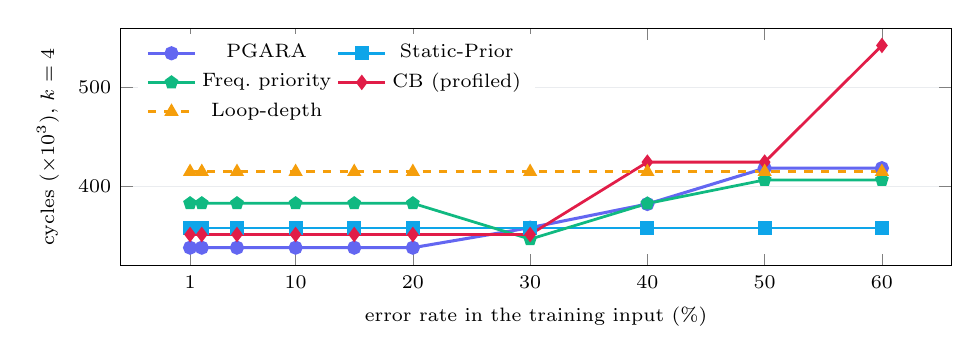
\begin{tikzpicture}
\begin{axis}[
  width=\columnwidth, height=46mm, xlabel={error rate in the training input (\%)},
  ylabel={cycles ($\times10^3$), $k=4$}, xtick={1,10,20,30,40,50,60},
  ymin=320, ymax=560,
  legend style={font=\scriptsize, at={(0.02,0.98)}, anchor=north west, draw=none, fill=white, legend columns=2},
  tick label style={font=\scriptsize}, label style={font=\scriptsize},
  ymajorgrids, grid style={draw=rule!80}]
\addplot[cPG, mark=*, line width=1.1pt] coordinates {(1,338.4) (2,338.4) (5,338.4) (10,338.4) (15,338.4) (20,338.4) (30,358.6) (40,382.5) (50,418.7) (60,418.7)};
\addplot[cSP, mark=square*, line width=1pt] coordinates {(1,358.2) (2,358.2) (5,358.2) (10,358.2) (15,358.2) (20,358.2) (30,358.2) (40,358.2) (50,358.2) (60,358.2)};
\addplot[cFP, mark=pentagon*, line width=1pt] coordinates {(1,383.2) (2,383.2) (5,383.2) (10,383.2) (15,383.2) (20,383.2) (30,347.0) (40,383.0) (50,406.8) (60,406.8)};
\addplot[cCBp, mark=diamond*, line width=1pt] coordinates {(1,351.7) (2,351.7) (5,351.7) (10,351.7) (15,351.7) (20,351.7) (30,351.7) (40,424.8) (50,424.8) (60,542.6)};
\addplot[cLD, dashed, mark=triangle*, mark options={solid}, line width=1pt] coordinates {(1,415.0) (2,415.0) (5,415.0) (10,415.0) (15,415.0) (20,415.0) (30,415.0) (40,415.0) (50,415.0) (60,415.0)};
\legend{\MG, Static-Prior, Freq.\ priority, CB (profiled), Loop-depth}
\end{axis}
\end{tikzpicture}
\caption{Rare-branch at $k=4$, measured on a test input with a 1\%
error rate, as the error rate of the training input grows. Linear scan
(516k cycles) is omitted for clarity.}
\label{fig:errsweep}
\end{figure}

\textit{Model constants.} Varying the register-access bonus $\csv$ over
$\{0,0.5,1,2\}$ and the forwarded-move cost $\cmv$ over $\{0,1,2\}$
changes \MG's geometric mean at $k=4$ only between 0.780 and 0.783
(Table~\ref{tab:costs}) and leaves it unchanged at $k=8$, so the
conclusions do not depend on these constants.

\begin{table}[t]
\centering
\caption{\MG's geometric-mean cycles relative to linear scan at $k=4$
for different model constants}
\label{tab:costs}
\footnotesize
\begin{tabular}{@{}lrrr@{}}
\toprule
$\csv$ & $\cmv=0$ & $\cmv=1$ & $\cmv=2$ \\
\midrule
0 & 0.7801 & 0.7803 & 0.7809 \\
0.5 & 0.7803 & 0.7817 & 0.7830 \\
1 & 0.7803 & 0.7817 & 0.7830 \\
2 & 0.7817 & 0.7830 & 0.7830 \\
\bottomrule
\end{tabular}
\end{table}

\textit{Realised versus optimal gain.} Over the 966 values of both
suites, the optimal policy $V^\ast$ would spill or reload inside the
live range for 189 values (20\%), but the realised gain
(\ref{eq:gain}) differs from the optimal-policy gain by only 0.05\% in
total, and by more than 1\% for 9 of the 809 values whose gain exceeds
one cycle. Bidding with either gain gives identical cycle counts in 48
of 51 configurations ($k\in\{3,4,8\}$) and at most 0.5\% difference in
the others. The bid of the first draft was therefore nearly harmless on
these programs, but the realised gain is the correct quantity and is
used throughout this version.

\textit{Coalition repair.} Concessions happen in practice: across the
119 configurations of the main study, 105 values conceded their
registers in the repair step, and the exclusion set of
Algorithm~\ref{alg:br} kept every one of them out of the second
best-response pass.

\subsection{Comparison with related approaches}

Table~\ref{tab:compare} positions \MG\ against the allocators it was
measured against and against the learned allocator
RL4ReAl~\cite{venkatakeerthy2023rl4real}, which we compare
qualitatively because it targets LLVM's back ends.

\begin{table}[t]
\centering
\caption{Qualitative comparison of allocation approaches}
\label{tab:compare}
\footnotesize
\setlength{\tabcolsep}{2.5pt}
\begin{tabular}{@{}>{\raggedright}p{20mm}>{\raggedright}p{22mm}>{\raggedright}p{14mm}>{\raggedright}p{9mm}>{\raggedright\arraybackslash}p{10mm}@{}}
\toprule
Approach & Decision basis & Measured profile & Training & Explain\-able \\
\midrule
Linear scan~\cite{poletto1999} & interval order & no & none & partly \\
Loop-depth priority~\cite{chow1990} & $10^{d}$ weights & no & none & yes \\
Chaitin--Briggs~\cite{briggs1994} & frequency-weighted spill cost & yes, as weights & none & partly \\
LLVM greedy~\cite{olesen2011greedy} & block-frequency spill weight, eviction & yes, as weights & none & partly \\
RL4ReAl~\cite{venkatakeerthy2023rl4real} & learned policy & indirectly & heavy & no \\
\MG\ (this work) & expected gain $G(v)$, auction & yes, in the MDP & none & yes (bids) \\
\bottomrule
\end{tabular}
\end{table}

\subsection{Answers to the research questions}
\label{sec:rq}

\textit{RQ1: Does profiling help?} Yes, moderately and where control
flow depends on data. With a representative training input, \MG\ is
1.1--3.1\% faster than the same engine with static priors at $k\le8$
(geometric mean over 17 programs) and executes 3--51\% fewer spill
operations; the gain reaches 14\% on scanner and 24\% on Levenshtein.
With a training input whose branch behaviour differs strongly from the
test input (above about 30\% error rate where the test has 1\%),
static priors are better.

\textit{RQ2: Does the MDP and auction formulation help beyond
profiling?} Yes. With the same profile, \MG\ is 3.3--4.8\% faster than
profiled-frequency priority, which differs only in replacing the MDP
gain by frequency-weighted access counts, and 1.2--4.5\% faster than
Chaitin--Briggs with profiled spill costs, at every $k\le8$ and on both
suites. The exception is extreme pressure ($k=3$) on three programs,
where Chaitin--Briggs packs registers better.

\textit{RQ3: How robust are the results?} The ranking is stable across
five test inputs per program, across the original and the independent
suites, and across the model constants. The benefit vanishes at
$k\ge16$, where no allocator except linear scan spills on these
programs, and it depends on a representative profile, with a
step-shaped degradation beyond a 20--40\% error rate.

\textit{RQ4: What does it cost?} Allocation takes 1--19\,ms per program
and grows roughly as $|V|^{1.35}$ with the number of values when live
ranges are short, but super-linearly, about $(\sum_v|L_v|)^{1.4}$, when live
ranges span hundreds of blocks. The profiling run costs more than
the allocation (27 times as much in total here) but is shared by all
register budgets and is the standard cost of any profile-guided build.

\subsection{Threats to validity}

\textit{Benchmarks.} The programs are small kernels: ten written for
this study and seven translated from MiBench and BEEBS. The translation
replaces bitwise operations with arithmetic, which changes their
instruction mix, and none of the programs is a large application.
$\theta$ is now tuned on a separate suite, but the cost constants of
Table~\ref{tab:params} are shared with the simulator.
\textit{Simulator.} Cycles come from a simulator with a fixed latency
table rather than from hardware; PG-RISC has no caches and no branch
predictor, so a spill always costs the same and a mispredicted branch
costs nothing extra, both of which favour a model whose costs are
exact. \textit{Register budgets.} The study covers $k\le32$, but the
benefit is confined to $k\le8$ on these programs; whether it appears at
realistic budgets depends on how often real code reaches that
pressure. \textit{Baselines.} The Chaitin--Briggs and profiled-frequency
baselines are our re-implementations on PG-RISC; they include
conservative coalescing, optimistic spilling and biased colouring but
not live-range splitting or the eviction and region splitting of
LLVM's greedy allocator, so a production allocator could be stronger.
\textit{Splitting.} The MDP's optimal policy may move a value between
register and memory inside its live range; the code generator does not
split live ranges, so this part of the policy is computed but not
realised, and the bid now uses the realised policy instead.

%% =====================================================================
\section{Conclusion and Future Work}
\label{sec:conclusion}

\MG\ allocates registers adaptively, guided by measured profiles, by
expected gain: a per-value Markov decision process over the live range,
evaluated with measured branch probabilities under the policy the code
generator realises, followed by a sealed-bid auction among
$\varphi$-web coalitions on the chordal SSA interference graph and
best-response dynamics to a Nash equilibrium. Existing allocators rank
values by static weights that cannot see data-dependent branches, scale
access counts by profiled frequencies without modelling where spills
and reloads occur, or learn opaque policies from large corpora.

The method makes the expected saving of each decision an explicit
number, needs no training, and costs milliseconds for ordinary
functions. It is embedded in a complete compiler, from an LL(1) grammar
and attribute-grammar semantic analysis through TAC, SSA and
optimisation to PG-RISC code and a simulator, with a web interface that
shows every phase.

On 17 programs and seven register budgets, all compiled programs match
the reference output. At $k=4$, \MG\ reduces geometric-mean cycles by
21.8\% relative to linear scan, 3.7\% relative to Chaitin--Briggs with
profile-weighted spill costs, 3.3\% relative to profiled-frequency
priority and 2.6\% relative to static priors, and it executes half as
many spill memory operations as linear scan. The ablations show that
profiling and the MDP gain each contribute, that the benefit is
concentrated on programs with skewed, data-dependent control flow and
on budgets of at most eight registers, and that it disappears when the
training profile misrepresents the test behaviour by a large margin.
Under extreme pressure ($k=3$), optimistic colouring with coalescing
still packs some programs better, and long live ranges make the
per-value linear systems the dominant compile-time cost.

Future work follows from these limitations: extend the MDP's policy
into live-range splitting in the code generator so that values can
move between register and memory inside a range; replace dense
elimination by banded or incremental solvers for long live ranges;
combine the gain with optimistic colouring when pressure is extreme;
replace whole-program averages with context-sensitive or phase-aware
profiles where the profile misleads; port the engine to a production
back end such as LLVM to evaluate it on standard suites and real
hardware; and combine measured profiles with learned profile
prediction~\cite{rotem2021pgo} when no representative input is
available.

%% =====================================================================
\section*{Author Contributions}

\begin{enumerate}
\item \textbf{Shreyans Chowdry}: core pipeline design, lexical and
syntax analysis, AST construction and intermediate code generation, and
the web GUI and pipeline visualisation interface, including the
Allocation view that displays gains, bids, coalitions and auction
rounds; in the \MG\ allocator, the edge profiler interface, the transition
matrices (\ref{eq:pprof})--(\ref{eq:pstat}), the block-frequency
solver (\ref{eq:freq}) and the hot-edge $\varphi$-web coalitions and
bids (\ref{eq:hot})--(\ref{eq:bid}).
\item \textbf{Samrender Singh Saini}: semantic analysis, scope
resolution and symbol table management; in the \MG\ allocator, the
interference graph, the maximum cardinality search and PEO
verification, and the sealed-bid auction and register binding
(Algorithm~\ref{alg:auction}).
\item \textbf{Karthikeya Jami}: SSA construction, the optimisation
engine and PG-RISC code generation; in the \MG\ allocator, the residency
MDP, policy iteration and the gain computation
(Algorithm~\ref{alg:gains}, (\ref{eq:reward})--(\ref{eq:gain})), and the
integration of the allocation with code generation.
\item \textbf{Abhishek Kumar}: runtime environment, simulator, test
suite and benchmarking; in the \MG\ allocator, best-response dynamics,
coalition repair (Algorithm~\ref{alg:br}), the baseline allocators and
ablations used in Section~\ref{sec:impl}, and the experiment scripts.
\item \textbf{Nishanth Kumar}: assisted with the user documentation and
with testing the web interface.
\end{enumerate}
All authors took part in the design discussions of the \MG\ allocator
and in the writing of this manuscript.

\section*{Acknowledgements}
The authors thank Bhuvaneswari M, School of Computer Science and
Engineering, Vellore Institute of Technology, for guidance on
recasting the allocator around stochastic dynamic programming and game
theory, and the reviewer of the first draft for comments that led to
the additional baselines and experiments in this version.

\section*{Funding}
This work received no external funding.

\section*{Competing Interests}
The authors declare no competing interests.

\section*{Data and Code Availability}
The compiler, the web interface, the three benchmark suites, the unit
tests, the experiment scripts and the raw results (JSON for all 1{,}428
configurations and every study in Section~\ref{sec:impl}) are publicly
available at \url{https://github.com/shreyans-chowdry/pgara}. The
results in this paper were produced from commit
\texttt{9b154888a712\allowbreak f99e2170fe\allowbreak a9a797388995\allowbreak d731f5}
(branch \texttt{draft2-revision}) with \texttt{python3 -m pgara.experiments};
the full-window screenshots of every view of the Compiler Studio are in
\texttt{docs/screenshots}, and a live instance of the interface is
hosted at \url{https://pgara.vercel.app}.

%% =====================================================================
\begin{thebibliography}{99}
\footnotesize

\bibitem{lattner2021mlir}
C.~Lattner, M.~Amini, U.~Bondhugula, A.~Cohen, A.~Davis, J.~Pienaar,
R.~Riddle, T.~Shpeisman, N.~Vasilache, and O.~Zinenko, ``MLIR: Scaling
compiler infrastructure for domain specific computation,'' in
\emph{Proc.\ IEEE/ACM Int.\ Symp.\ Code Generation and Optimization
(CGO)}, 2021, pp.~2--14.

\bibitem{wang2018ml}
Z.~Wang and M.~O'Boyle, ``Machine learning in compiler optimization,''
\emph{Proc.\ IEEE}, vol.~106, no.~11, pp.~1879--1901, 2018.

\bibitem{ashouri2018survey}
A.~H. Ashouri, W.~Killian, J.~Cavazos, G.~Palermo, and C.~Silvano, ``A
survey on compiler autotuning using machine learning,'' \emph{ACM
Comput.\ Surv.}, vol.~51, no.~5, art.~96, 2018.

\bibitem{leather2020ml}
H.~Leather and C.~Cummins, ``Machine learning in compilers: Past,
present and future,'' in \emph{Proc.\ Forum for Specification and
Design Languages (FDL)}, 2020.

\bibitem{cytron1991ssa}
R.~Cytron, J.~Ferrante, B.~K. Rosen, M.~N. Wegman, and F.~K. Zadeck,
``Efficiently computing static single assignment form and the control
dependence graph,'' \emph{ACM Trans.\ Program.\ Lang.\ Syst.}, vol.~13,
no.~4, pp.~451--490, 1991.

\bibitem{rastello2022ssa}
F.~Rastello and F.~Bouchez~Tichadou, Eds., \emph{SSA-based Compiler
Design}. Cham, Switzerland: Springer, 2022.

\bibitem{cooper2022eac}
K.~D. Cooper and L.~Torczon, \emph{Engineering a Compiler}, 3rd~ed.
Cambridge, MA, USA: Morgan Kaufmann, 2022.

\bibitem{aho2006dragon}
A.~V. Aho, M.~S. Lam, R.~Sethi, and J.~D. Ullman, \emph{Compilers:
Principles, Techniques, and Tools}, 2nd~ed. Boston, MA, USA:
Addison-Wesley, 2006.

\bibitem{chaitin1982}
G.~J. Chaitin, ``Register allocation \& spilling via graph coloring,''
in \emph{Proc.\ SIGPLAN Symp.\ Compiler Construction}, 1982,
pp.~98--105.

\bibitem{chow1990}
F.~C. Chow and J.~L. Hennessy, ``The priority-based coloring approach
to register allocation,'' \emph{ACM Trans.\ Program.\ Lang.\ Syst.},
vol.~12, no.~4, pp.~501--536, 1990.

\bibitem{olesen2011greedy}
J.~Olesen, ``Greedy register allocation in LLVM 3.0,'' LLVM Project
Blog, Sep.~2011. [Online]. Available:
\url{https://blog.llvm.org/2011/09/greedy-register-allocation-in-llvm-30.html}

\bibitem{llvmbfi}
LLVM Project, ``LLVM block frequency terminology,'' LLVM documentation.
[Online]. Available:
\url{https://llvm.org/docs/BlockFrequencyTerminology.html}

\bibitem{poletto1999}
M.~Poletto and V.~Sarkar, ``Linear scan register allocation,''
\emph{ACM Trans.\ Program.\ Lang.\ Syst.}, vol.~21, no.~5,
pp.~895--913, 1999.

\bibitem{hack2006ssa}
S.~Hack, D.~Grund, and G.~Goos, ``Register allocation for programs in
SSA-form,'' in \emph{Proc.\ Int.\ Conf.\ Compiler Construction (CC)},
LNCS~3923, 2006, pp.~247--262.

\bibitem{hack2006ipl}
S.~Hack and G.~Goos, ``Optimal register allocation for SSA-form
programs in polynomial time,'' \emph{Inf.\ Process.\ Lett.}, vol.~98,
no.~4, pp.~150--155, 2006.

\bibitem{lozano2019toplas}
R.~Castañeda Lozano, M.~Carlsson, G.~Hjort Blindell, and C.~Schulte,
``Combinatorial register allocation and instruction scheduling,''
\emph{ACM Trans.\ Program.\ Lang.\ Syst.}, vol.~41, no.~3, art.~17,
2019.

\bibitem{lozano2019survey}
R.~Castañeda Lozano and C.~Schulte, ``Survey on combinatorial register
allocation and instruction scheduling,'' \emph{ACM Comput.\ Surv.},
vol.~52, no.~3, art.~62, 2019.

\bibitem{trofin2021mlgo}
M.~Trofin, Y.~Qian, E.~Brevdo, Z.~Lin, K.~Choromanski, and D.~Li,
``MLGO: A machine learning guided compiler optimizations framework,''
arXiv:2101.04808, 2021.

\bibitem{venkatakeerthy2023rl4real}
S.~VenkataKeerthy, S.~Jain, A.~Kundu, R.~Aggarwal, A.~Cohen, and
R.~Upadrasta, ``RL4ReAl: Reinforcement learning for register
allocation,'' in \emph{Proc.\ ACM SIGPLAN Int.\ Conf.\ Compiler
Construction (CC)}, 2023, pp.~133--144.

\bibitem{venkatakeerthy2020ir2vec}
S.~VenkataKeerthy, R.~Aggarwal, S.~Jain, M.~S. Desarkar, R.~Upadrasta,
and Y.~N. Srikant, ``IR2Vec: LLVM IR based scalable program
embeddings,'' \emph{ACM Trans.\ Archit.\ Code Optim.}, vol.~17, no.~4,
art.~32, 2020.

\bibitem{cummins2022compilergym}
C.~Cummins, B.~Wasti, J.~Guo, B.~Cui, J.~Ansel, S.~Gomez, S.~Jain,
J.~Liu, O.~Teytaud, B.~Steiner, Y.~Tian, and H.~Leather, ``CompilerGym:
Robust, performant compiler optimization environments for AI
research,'' in \emph{Proc.\ IEEE/ACM Int.\ Symp.\ Code Generation and
Optimization (CGO)}, 2022, pp.~92--105.

\bibitem{cummins2021programl}
C.~Cummins, Z.~V. Fisches, T.~Ben-Nun, T.~Hoefler, M.~F.~P. O'Boyle,
and H.~Leather, ``ProGraML: A graph-based program representation for
data flow analysis and compiler optimizations,'' in \emph{Proc.\ Int.\
Conf.\ Machine Learning (ICML)}, PMLR~139, 2021, pp.~2244--2253.

\bibitem{panchenko2019bolt}
M.~Panchenko, R.~Auler, B.~Nell, and G.~Ottoni, ``BOLT: A practical
binary optimizer for data centers and beyond,'' in \emph{Proc.\
IEEE/ACM Int.\ Symp.\ Code Generation and Optimization (CGO)}, 2019,
pp.~2--14.

\bibitem{shen2023propeller}
H.~Shen, K.~Pszeniczny, R.~Lavaee, S.~Kumar, S.~Tallam, and X.~D. Li,
``Propeller: A profile guided, relinking optimizer for warehouse-scale
applications,'' in \emph{Proc.\ ACM Int.\ Conf.\ Architectural Support
for Programming Languages and Operating Systems (ASPLOS)}, 2023.

\bibitem{rotem2021pgo}
N.~Rotem and C.~Cummins, ``Profile guided optimization without
profiles: A machine learning approach,'' arXiv:2112.14679, 2021.

\bibitem{wagner1994}
T.~A. Wagner, V.~Maverick, S.~L. Graham, and M.~A. Harrison,
``Accurate static estimators for program optimization,'' in
\emph{Proc.\ ACM SIGPLAN Conf.\ Programming Language Design and
Implementation (PLDI)}, 1994, pp.~85--96.

\bibitem{wu1994}
Y.~Wu and J.~R. Larus, ``Static branch frequency and program profile
analysis,'' in \emph{Proc.\ 27th Annu.\ Int.\ Symp.\ Microarchitecture
(MICRO)}, 1994, pp.~1--11.

\bibitem{wall1991}
D.~W. Wall, ``Predicting program behavior using real or estimated
profiles,'' in \emph{Proc.\ ACM SIGPLAN Conf.\ Programming Language
Design and Implementation (PLDI)}, 1991, pp.~59--70.

\bibitem{callahan1991}
D.~Callahan and B.~Koblenz, ``Register allocation via hierarchical
graph coloring,'' in \emph{Proc.\ ACM SIGPLAN Conf.\ Programming Language
Design and Implementation (PLDI)}, 1991, pp.~192--203.

\bibitem{koes2006}
D.~R. Koes and S.~C. Goldstein, ``A global progressive register
allocator,'' in \emph{Proc.\ ACM SIGPLAN Conf.\ Programming Language
Design and Implementation (PLDI)}, 2006, pp.~204--215.

\bibitem{sutton2018rl}
R.~S. Sutton and A.~G. Barto, \emph{Reinforcement Learning: An
Introduction}, 2nd~ed. Cambridge, MA, USA: MIT Press, 2018.

\bibitem{puterman1994}
M.~L. Puterman, \emph{Markov Decision Processes: Discrete Stochastic
Dynamic Programming}. New York, NY, USA: Wiley, 1994.

\bibitem{bertsekas2019}
D.~P. Bertsekas, \emph{Reinforcement Learning and Optimal Control}.
Belmont, MA, USA: Athena Scientific, 2019.

\bibitem{howard1960}
R.~A. Howard, \emph{Dynamic Programming and Markov Processes}.
Cambridge, MA, USA: MIT Press, 1960.

\bibitem{shapley1953}
L.~S. Shapley, ``A value for $n$-person games,'' in \emph{Contributions
to the Theory of Games II}, Annals of Mathematics Studies~28.
Princeton, NJ, USA: Princeton Univ.\ Press, 1953, pp.~307--317.

\bibitem{vickrey1961}
W.~Vickrey, ``Counterspeculation, auctions, and competitive sealed
tenders,'' \emph{J.~Finance}, vol.~16, no.~1, pp.~8--37, 1961.

\bibitem{tarjan1984}
R.~E. Tarjan and M.~Yannakakis, ``Simple linear-time algorithms to test
chordality of graphs, test acyclicity of hypergraphs, and selectively
reduce acyclic hypergraphs,'' \emph{SIAM J.\ Comput.}, vol.~13, no.~3,
pp.~566--579, 1984.

\bibitem{rosenthal1973}
R.~W. Rosenthal, ``A class of games possessing pure-strategy Nash
equilibria,'' \emph{Int.\ J.\ Game Theory}, vol.~2, no.~1, pp.~65--67,
1973.

\bibitem{nisan2007agt}
N.~Nisan, T.~Roughgarden, {\'E}.~Tardos, and V.~V. Vazirani, Eds.,
\emph{Algorithmic Game Theory}. Cambridge, U.K.: Cambridge Univ.\
Press, 2007.

\bibitem{jain2022posetrl}
S.~Jain, Y.~Andaluri, S.~VenkataKeerthy, and R.~Upadrasta, ``POSET-RL:
Phase ordering for optimizing size and execution time using
reinforcement learning,'' in \emph{Proc.\ IEEE Int.\ Symp.\ Performance
Analysis of Systems and Software (ISPASS)}, 2022, pp.~121--131.

\bibitem{hajali2020neurovectorizer}
A.~Haj-Ali, N.~K. Ahmed, T.~Willke, Y.~S. Shao, K.~Asanovic, and
I.~Stoica, ``NeuroVectorizer: End-to-end vectorization with deep
reinforcement learning,'' in \emph{Proc.\ IEEE/ACM Int.\ Symp.\ Code
Generation and Optimization (CGO)}, 2020, pp.~242--255.

\bibitem{cummins2025llmcompiler}
C.~Cummins, V.~Seeker, D.~Grubisic, B.~Rozi{\`e}re, J.~Gehring,
G.~Synnaeve, and H.~Leather, ``LLM Compiler: Foundation language models
for compiler optimization,'' in \emph{Proc.\ 34th ACM SIGPLAN Int.\
Conf.\ Compiler Construction (CC)}, 2025.

\bibitem{briggs1994}
P.~Briggs, K.~D. Cooper, and L.~Torczon, ``Improvements to graph
coloring register allocation,'' \emph{ACM Trans.\ Program.\ Lang.\
Syst.}, vol.~16, no.~3, pp.~428--455, 1994.

\bibitem{george1996}
L.~George and A.~W. Appel, ``Iterated register coalescing,'' \emph{ACM
Trans.\ Program.\ Lang.\ Syst.}, vol.~18, no.~3, pp.~300--324, 1996.

\bibitem{lueh2000}
G.-Y. Lueh, T.~Gross, and A.-R. Adl-Tabatabai, ``Fusion-based register
allocation,'' \emph{ACM Trans.\ Program.\ Lang.\ Syst.}, vol.~22,
no.~3, pp.~431--470, 2000.

\bibitem{knuth1965lr}
D.~E. Knuth, ``On the translation of languages from left to right,''
\emph{Inf.\ Control}, vol.~8, no.~6, pp.~607--639, 1965.

\bibitem{lewis1968}
P.~M. Lewis and R.~E. Stearns, ``Syntax-directed transduction,''
\emph{J.~ACM}, vol.~15, no.~3, pp.~465--488, 1968.

\bibitem{knuth1968attr}
D.~E. Knuth, ``Semantics of context-free languages,'' \emph{Math.\
Syst.\ Theory}, vol.~2, no.~2, pp.~127--145, 1968.

\bibitem{cooper2001dom}
K.~D. Cooper, T.~J. Harvey, and K.~Kennedy, ``A simple, fast dominance
algorithm,'' Rice Univ., Houston, TX, USA, Tech.\ Rep., 2001.

\bibitem{wegman1991sccp}
M.~N. Wegman and F.~K. Zadeck, ``Constant propagation with conditional
branches,'' \emph{ACM Trans.\ Program.\ Lang.\ Syst.}, vol.~13, no.~2,
pp.~181--210, 1991.

\bibitem{bellman1957}
R.~Bellman, \emph{Dynamic Programming}. Princeton, NJ, USA: Princeton
Univ.\ Press, 1957.

\bibitem{panagopoulou2008}
P.~N. Panagopoulou and P.~G. Spirakis, ``A game theoretic approach for
efficient graph coloring,'' in \emph{Proc.\ Int.\ Symp.\ Algorithms and
Computation (ISAAC)}, LNCS 5369, 2008, pp.~183--195.

\bibitem{monderer1996}
D.~Monderer and L.~S. Shapley, ``Potential games,'' \emph{Games Econ.\
Behav.}, vol.~14, no.~1, pp.~124--143, 1996.

\bibitem{python}
Python Software Foundation, ``Python 3 documentation,'' 2024.
[Online]. Available: \url{https://docs.python.org/3/}

\bibitem{coveragepy}
N.~Batchelder \emph{et~al.}, ``Coverage.py: Code coverage measurement
for Python.'' [Online]. Available: \url{https://coverage.readthedocs.io/}

\bibitem{playwright}
Microsoft, ``Playwright: Fast and reliable end-to-end testing for
modern web apps,'' 2024. [Online]. Available:
\url{https://playwright.dev/}

\bibitem{guthaus2001mibench}
M.~R. Guthaus, J.~S. Ringenberg, D.~Ernst, T.~M. Austin, T.~Mudge, and
R.~B. Brown, ``MiBench: A free, commercially representative embedded
benchmark suite,'' in \emph{Proc.\ IEEE Int.\ Workshop Workload
Characterization (WWC-4)}, 2001, pp.~3--14.

\bibitem{pallister2013beebs}
J.~Pallister, S.~Hollis, and J.~Bennett, ``BEEBS: Open benchmarks for
energy measurements on embedded platforms,'' arXiv:1308.5174, 2013.

\end{thebibliography}

\clearpage
\newcommand{\photoplaceholder}{\fbox{\parbox[c][1.17in][c]{0.93in}{\centering\scriptsize Photograph\\to be added}}}

\begin{IEEEbiography}[{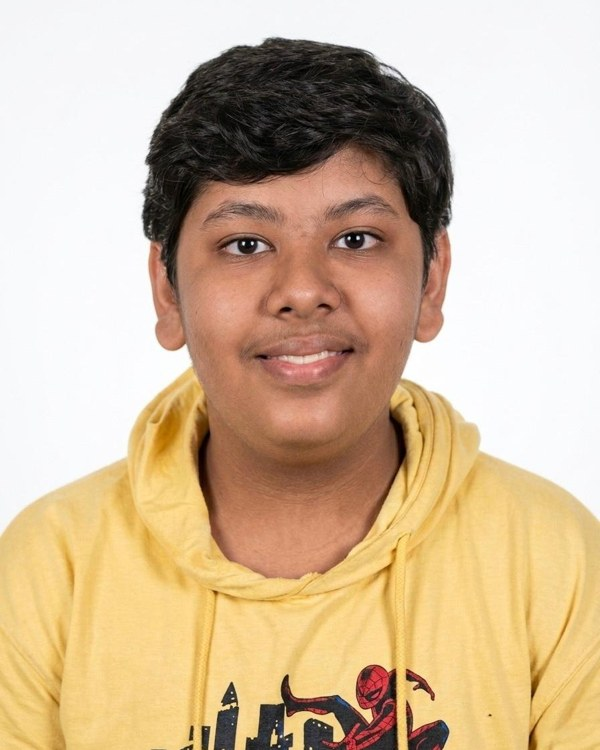
\includegraphics[width=1in,height=1.25in,clip,keepaspectratio]{photos/shreyans.jpg}}]{Shreyans Chowdry}
is pursuing the B.Tech.\ degree in Computer Science and Engineering
with a specialisation in Data Science at the Vellore Institute of
Technology, Vellore, India. His interests include compilers, applied
artificial intelligence and full-stack software engineering. In this
work he designed the core compiler pipeline (lexer, LL(1) grammar and
parser, AST and three-address code), built the web interface, and
developed the profile-derived transition model and the $\varphi$-web
coalitions of the \MG\ allocator.
\end{IEEEbiography}

\begin{IEEEbiography}[{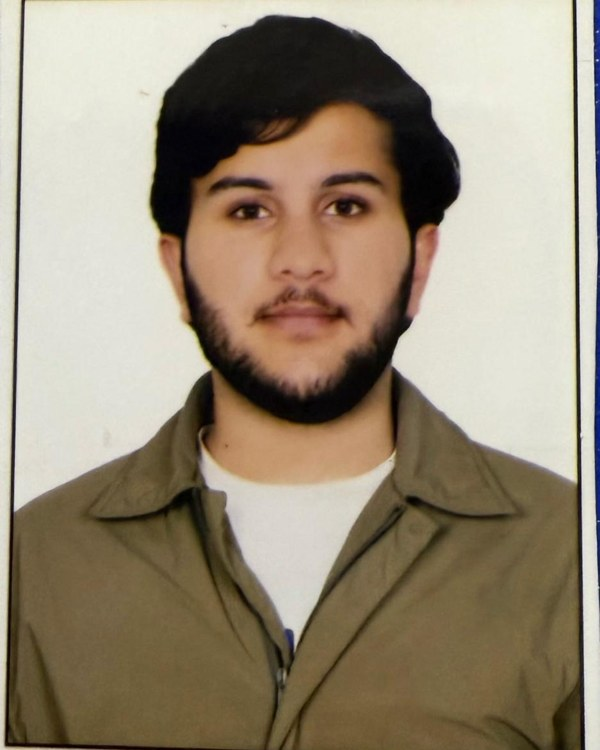
\includegraphics[width=1in,height=1.25in,clip,keepaspectratio]{photos/samrender.jpg}}]{Samrender Singh Saini}
is pursuing the B.Tech.\ degree in Computer Science and Engineering at
the Vellore Institute of Technology, Vellore, India. In this work he
developed the semantic analysis, scope resolution and symbol table
management of the compiler, and the interference graph, maximum
cardinality search and sealed-bid auction of the \MG\ allocator.
\end{IEEEbiography}

\begin{IEEEbiography}[{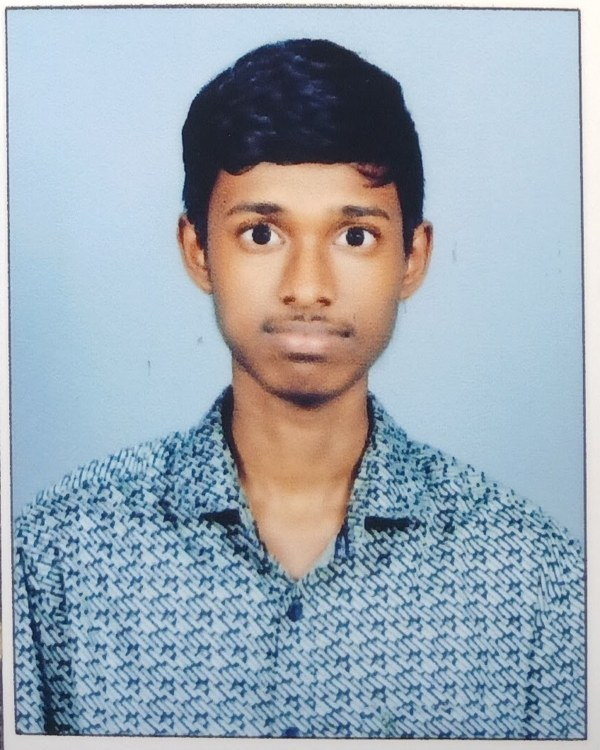
\includegraphics[width=1in,height=1.25in,clip,keepaspectratio]{photos/karthikeya.jpg}}]{Karthikeya Jami}
is pursuing the B.Tech.\ degree in Computer Science and Engineering at
the Vellore Institute of Technology, Vellore, India. In this work he
developed SSA construction, the optimiser and PG-RISC code generation,
and the residency MDP, policy iteration and gain computation of the
\MG\ allocator.
\end{IEEEbiography}

\begin{IEEEbiography}[{
\includegraphics[width=1in,height=1.25in,clip,keepaspectratio]{photos/abhishek.jpg}}]{Abhishek Kumar}
is pursuing the B.Tech.\ degree in Computer Science and Engineering at
the Vellore Institute of Technology, Vellore, India. In this work he
developed the reference interpreter, the cycle-counting simulator, the
test suite and the benchmark harness, and the best-response dynamics,
coalition repair and baseline allocators of the \MG\ allocator.
\end{IEEEbiography}

\begin{IEEEbiography}[{\photoplaceholder}]{Nishanth Kumar}
is pursuing the B.Tech.\ degree in Computer Science and Engineering
(Artificial Intelligence and Machine Learning) at the Vellore Institute
of Technology, Vellore, India. In this work he assisted with the
documentation and with testing the web interface.
\end{IEEEbiography}

\EOD

\end{document}
